\documentclass[a4paper, 14pt]{extarticle}
%\usepackage[utf8]{inputenc}
%\usepackage[english,russian]{babel}
%\usepackage{indentfirst}

%\usepackage{graphicx}
%\usepackage{float}
%\usepackage{wrapfig}
%\graphicspath{{images/}}

\usepackage[T2A]{fontenc}
\usepackage[utf8]{inputenc}%включаем свою кодировку: koi8-r или utf8 в UNIX, cp1251 в Windows
\usepackage[english,russian]{babel}%используем русский и английский языки с переносами
\usepackage{amssymb,amsfonts,amsmath,mathtext,enumerate,float} %подключаем нужные пакеты расширений
\usepackage{graphicx}
\usepackage{cmap}
\usepackage{verbatim}
\graphicspath{{images/}}%путь к рисункам
\bibliographystyle{gost-numeric.bbx}
\usepackage[parentracker=true,
            backend=biber,
            bibencoding=utf8,
            style=numeric-comp,
            language=auto,
            autolang=other,
            citestyle=gost-numeric,
            defernumbers=true,
            bibstyle=gost-numeric,
            sorting=none
]{biblatex}
\addbibresource{infrastructure/bibliography.bib}
\usepackage{geometry} % Меняем поля страницы
\geometry{left=3cm}% левое поле
\geometry{right=2cm}% правое поле
\geometry{top=2cm}% верхнее поле
\geometry{bottom=2cm}% нижнее поле
\tolerance=3000
\geometry{marginparwidth=2.5cm} % Ширина заметок на полях.
\usepackage{biblatex}
\usepackage{microtype}
%\usepackage{cite}

\makeatletter
\renewcommand{\@biblabel}[1]{#1.} % Заменяем библиографию с квадратных скобок на точку:
\makeatother

\usepackage{float}
\usepackage{xcolor}
\usepackage{marginnote}
\reversemarginpar % Перенос заметок с правого поля на левое.
\usepackage{hyperref}
\usepackage{tabularx}
\usepackage{amsmath}

% Полезные типы колонок: колонки с выравниваем влево/по центру/справа
% фиксированной ширины (как p{}, но не justify).
\newcolumntype{L}[1]{>{\raggedright\let\newline\\\arraybackslash\hspace{0pt}}m{#1}}
\newcolumntype{C}[1]{>{\centering\let\newline\\\arraybackslash\hspace{0pt}}m{#1}}
\newcolumntype{R}[1]{>{\raggedleft\let\newline\\\arraybackslash\hspace{0pt}}m{#1}}

% Колонки для tabularx
\newcolumntype{E}[1]{>{\hsize=#1\hsize\raggedright\arraybackslash}X}%
\newcolumntype{F}[1]{>{\hsize=#1\hsize\centering\arraybackslash}X}%
\newcolumntype{G}[1]{>{\hsize=#1\hsize\raggedleft\arraybackslash}X}%
%\newcolumntype{C}[2]{>{\hsize=#1\hsize\columncolor{#2}\centering\arraybackslash}X}%

\usepackage{indentfirst}
\usepackage{setspace}
\setstretch{1.5}

\usepackage{enumitem}
\setlist{nolistsep}

% % % % % % % % % % % % % % % % % % %
% Нумерация абзацев
% % % % % % % % % % % % % % % % % % %

\renewcommand{\theenumi}{\arabic{enumi}}% Меняем везде перечисления на цифра.цифра
%\renewcommand{\labelenumi}{\arabic{enumi}}% Меняем везде перечисления на цифра.цифра
\renewcommand{\theenumii}{.\arabic{enumii}}% Меняем везде перечисления на цифра.цифра
\renewcommand{\labelenumii}{\arabic{enumi}.\arabic{enumii}.}% Меняем везде перечисления на цифра.цифра
\renewcommand{\theenumiii}{.\arabic{enumiii}}% Меняем везде перечисления на цифра.цифра
\renewcommand{\labelenumiii}{\arabic{enumi}.\arabic{enumii}.\arabic{enumiii}.}% Меняем везде перечисления на цифра.цифра

\renewcommand{\thesection}{\arabic{section}}
%\renewcommand{\thesubsection}{\arabic{subsection}}
%\renewcommand{\thesubsubsection}{\arabic{subsubsection}}
\setlength{\intextsep}{1.75\intextsep}
\setcounter{secnumdepth}{5}
\setcounter{tocdepth}{5}
%\addtolength{\parskip}{8pt}


% % % % % % % % % % % % % % % % % % %
% Новые команды
% % % % % % % % % % % % % % % % % % %

\newcommand{\off}[1]{{\color{gray}#1}}

%\newcommand{\todo}[1]{\marginpar{\color{red} \footnotesize #1}}
%\newcommand{\todonote}[1]{\todo{#1}}
%\newcommand{\toask}[1]{\marginpar{\color{blue} \footnotesize #1}}

%\newcommand{\todo}[1]{}
%\newcommand{\todonote}[1]{{\color{red}#1}}
%\newcommand{\toask}[1]{{\color{blue}#1}}

\newcommand{\todo}[1]{}
\newcommand{\todonote}[1]{}
\newcommand{\toask}[1]{}


\newcommand{\comm}[1]{\marginpar{\color{red}\Large \textbf{!!}}}
\newcommand{\alt}[2]{$\overset{\text{#2}}{\text{#1}}$}
\newcommand{\tweakedsim}{{\raise.17ex\hbox{$\scriptstyle\sim$}}}
\newcommand{\ceil}[1]{\left\lceil#1\right\rceil}
\newcommand{\abs}[1]{\left|#1\right|}
\renewcommand{\phi}{\varphi}

\begin{document}
\newcommand{\fnt}[1]{\fontsize{#1}{\baselineskip}\selectfont}
% Ставим геометрию для титульной страницы.
\newgeometry{left=3cm,right=1.5cm,top=2cm,bottom=2cm}

% Просто информация. Нигде в странице не используется, но зато попадёт в pdf info.
\author{Мингулов К.\:Т.}
\title{Пакет DREAM: автоматизация метода многопетлевых вычислений, основанного на рекуррентных соотношениях по размерности пространства-времени}
\date{2022 г.}
\begin{titlepage}
\begin{spacing}{1}
%%%%%%%%%%%%%%%%%%%%%%%%%%%%%%%%%%%%%%%%%%%%%%%%%%%%%%%%%%%%%%%%%%%%%%%%%%%%%%%%

\begin{center}
    {\fnt{10.5} МИНИСТЕРСТВО НАУКИ И ВЫСШЕГО ОБРАЗОВАНИЯ РОССИЙСКОЙ ФЕДЕРАЦИИ} \\
        \vspace{0.3\baselineskip}
    {\fnt{10.5} ФЕДЕРАЛЬНОЕ ГОСУДАРСТВЕННОЕ АВТОНОМНОЕ ОБРАЗОВАТЕЛЬНОЕ \\
		\vspace{-0.3\baselineskip}
		УЧРЕЖДЕНИЕ ВЫСШЕГО ОБРАЗОВАНИЯ} \\
        \vspace{0.3\baselineskip}
    {\fnt{10.5} <<\mbox{\textls[-18]{НОВОСИБИРСКИЙ НАЦИОНАЛЬНЫЙ ИССЛЕДОВАТЕЛЬСКИЙ ГОСУДАРСТВЕННЫЙ}}\\
		\vspace{-0.3\baselineskip}
		УНИВЕРСИТЕТ>> (НОВОСИБИРСКИЙ ГОСУДАРСТВЕННЫЙ УНИВЕРСИТЕТ, НГУ)}
\end{center}

%%%%%%%%%%%%%%%%%%%%%%%%%%%%%%%%%%%%%%%%%%%%%%%%%%%%%%%%%%%%%%%%%%%%%%%%%%%%%%%%

\vspace{0.5\baselineskip}

\noindent
{\fnt{11}Факультет}
$\overset{\text{\fnt{11}\textbf{ФИЗИЧЕСКИЙ}}\phantom{\hspace{10.9cm}}}{\underline{\hspace{0.88\textwidth}}}$

\vspace{0.3\baselineskip}

\noindent
{\fnt{11}Кафедра}
$\overset{\text{\fnt{11}\textbf{ФИЗИКО-ТЕХНИЧЕСКОЙ ИНФОРМАТИКИ}}\phantom{\hspace{4.8cm}}}{\underline{\hspace{0.895\textwidth}}}$

\vspace{1\baselineskip}

\noindent
{\fnt{11}Направление подготовки}
$\overset{\text{\fnt{11}\textbf{03.03.02 ФИЗИКА}}\phantom{\hspace{8cm}}}{\underline{\hspace{0.73\textwidth}}}$

\vspace{0.3\baselineskip}

\noindent
{\fnt{11}Образовательная программа}
$\overset{\text{\fnt{11}\textbf{МАГИСТРАТУРА}}\phantom{\hspace{7.3cm}}}{\underline{\hspace{0.689\textwidth}}}$

%%%%%%%%%%%%%%%%%%%%%%%%%%%%%%%%%%%%%%%%%%%%%%%%%%%%%%%%%%%%%%%%%%%%%%%%%%%%%%%%

\vspace{\baselineskip}

\begin{center}\bfseries
    {\fnt{11} ВЫПУСКНАЯ КВАЛИФИКАЦИОННАЯ РАБОТА} \\
        \vspace{0\baselineskip}
    %{\fnt{11} МАГИСТЕРСКАЯ ДИССЕРТАЦИЯ}
\end{center}

%%%%%%%%%%%%%%%%%%%%%%%%%%%%%%%%%%%%%%%%%%%%%%%%%%%%%%%%%%%%%%%%%%%%%%%%%%%%%%%%

\vspace{0.3\baselineskip}

\noindent
$\overset{\text{\fnt{11}Андреев Андрей Андреевич}}
{\underset{\text{\fnt{9}(Фамилия, Имя, Отчество автора)}}{\underline{\hspace{\textwidth}}}}$

%%%%%%%%%%%%%%%%%%%%%%%%%%%%%%%%%%%%%%%%%%%%%%%%%%%%%%%%%%%%%%%%%%%%%%%%%%%%%%%%

\vspace{\baselineskip}

\noindent
{\fnt{11}Тема работы}
$\overset{\text{\fnt{11}Блок упаковки данных для системы FEX модуля LASP жидкоаргонового }}{\underline{\hspace{0.855\textwidth}}}$

\noindent
$\overset{\text{\fnt{11}калориметра детектора ATLAS}}{\underline{\hspace{\textwidth}}}$

\noindent
$\overset{\text{\fnt{11}}}{\underline{\hspace{\textwidth}}}$

%%%%%%%%%%%%%%%%%%%%%%%%%%%%%%%%%%%%%%%%%%%%%%%%%%%%%%%%%%%%%%%%%%%%%%%%%%%%%%%%

\vspace{2\baselineskip}

\noindent
\begin{tabular}{@{}p{0.5\textwidth}@{}@{}R{0.5\textwidth}@{}}
\fnt{11}\textbf{<<К защите допущена>>} &  \\
\fnt{11}Декан ФФ НГУ                   & \fnt{11}\textbf{Научный руководитель} \\
\fnt{11}д.ф.-м.н.           & \fnt{11}канд. техн. наук \\
\fnt{11}зав. лаб. 3-2 ИЯФ СО РАН               & \fnt{11}зав. сек. 3-12 ИЯФ СО РАН \\
$\overset{\text{\fnt{11}Блинов В.\,Е.}}{\underset{\text{\fnt{8}(фамилия, И., О.)}}{\underline{\hspace{0.225\textwidth}}}}
\overset{\text{\fnt{11}/}}{}
\overset{\text{\fnt{11}}}{\underset{\text{\fnt{8}(подпись, МП)}}{\underline{\hspace{0.125\textwidth}}}}$ &
$\overset{\text{\fnt{11}Жуланов В.\,В.}}{\underset{\text{\fnt{8}(фамилия, И.,О.)}}{\underline{\hspace{0.225\textwidth}}}}
\overset{\text{\fnt{11}/}}{}
\overset{\text{\fnt{11}}}{\underset{\text{\fnt{8}(подпись, МП)}}{\underline{\hspace{0.125\textwidth}}}}$ \\
$\overset{\text{\fnt{11}<<}}{}
\overset{\text{\fnt{11}}}{\underline{\hspace{0.05\textwidth}}}
\overset{\text{\fnt{11}>>}}{}
\overset{\text{\fnt{11}}}{\underline{\hspace{0.215\textwidth}}}
\overset{\text{\fnt{11}2022 г.}}{}$ &
$\overset{\text{\fnt{11}<<}}{}
\overset{\text{\fnt{11}}}{\underline{\hspace{0.05\textwidth}}}
\overset{\text{\fnt{11}>>}}{}
\overset{\text{\fnt{11}}}{\underline{\hspace{0.215\textwidth}}}
\overset{\text{\fnt{11}2022 г.}}{}$
\end{tabular}

%%%%%%%%%%%%%%%%%%%%%%%%%%%%%%%%%%%%%%%%%%%%%%%%%%%%%%%%%%%%%%%%%%%%%%%%%%%%%%%%

\vspace{1.5\baselineskip}

\begin{flushright}
\fnt{11}
$\overset{\text{\fnt{11}Дата защиты: <<}}{}
\overset{\text{\fnt{11}}}{\underline{\hspace{0.05\textwidth}}}
\overset{\text{\fnt{11}>>}}{}
\overset{\text{\fnt{11}}}{\underline{\hspace{0.215\textwidth}}}
\overset{\text{\fnt{11}2022 г.}}{}$
\end{flushright}

%%%%%%%%%%%%%%%%%%%%%%%%%%%%%%%%%%%%%%%%%%%%%%%%%%%%%%%%%%%%%%%%%%%%%%%%%%%%%%%%

\vfill

\begin{center}
    \fnt{11} Новосибирск, 2022
\end{center}

\end{spacing}
\end{titlepage}

\restoregeometry


\tableofcontents
\thispagestyle{empty}
\newpage

\setcounter{page}{3}
\section*{Введение}
\addcontentsline{toc}{section}{Введение}
    ATLAS -- это один из четырёх основных экспериментов на Большом Адронном коллайдере (БАК). Эксперимент проводится на одноимённом детекторе, предназначенном для исследования протон-протонных столкновений и столкновений тяжелых ионов. Экспериментальные данные, полученные на многоцелевом детекторе ATLAS, используются для дальнейшего изучения свойств бозона Хиггса, поиска суперсимметричных частиц и широкого набора других задач.\par

В рамках второй фазы обновления системы жидкоаргоновых детекторов ATLAS ведётся проектирование совершенно новой системы считывающей электроники, которая будет установлена в период третьего длительного отключения БАК (2024 -- 2026 гг.). Это позволит расширить возможности эксперимента после модернизации Большого Адронного коллайдера, в результате которой ожидается значительное повышение мгновенной светимости до $7,5*10^{34} \text{см}^{-2}\text{c}^{-1}$ с целью обеспечения интегральной светимости $4000 \text{фб}^{-1}$ через период около 12 лет. Это позволит использовать БАК для исследования "новой физики", лежащей за границами Стандартной Модели.\par

Важным компонентом новой считывающей системы будет являться сигнальный процессор LASP (Liquid Argon Signal Processor), реализующий приём оцифрованных сигналов, цифровую фильтрацию и буферизацию данных до момента принятия решения триггерной системы. В основе данного модуля будет работать микросхема программируемой логики (ПЛИС). В настоящее время ведётся активная разработка этого процессора, частью которой является данная работа.\par

    \newpage

\section{Эксперимент ATLAS}
    Эксперимент ATLAS является одним из четырёх основных экспериментов на Большом адронном коллайдепре(БАК). Он проводится на одноимённом детекторе общего назначения, предназначенном для изучения протон-протонных столкновений, а также столкновений тяжелых ионов. С помощью детектора ATLAS проводится широкий спектр исследований в области физики элементарных частиц от поиска бозона Хиггса, до попыток обнаружения частиц, которые могут составлять тёмную материю. Кроме того, одним из важных направлений является поиск новых физических явлений, которые не описываются стандартной моделью.\par

\subsection{Калориметрическая система}
Калориметрическая система детектора ATLAS имеет ключевую роль в измерении энергии и положения электронов, фотонов и заряженных адронов. Система калориметров является составной и состоит из четырёх основных частей \parencite{tdr_green} (рис. \ref{fig:atlas_cal}):
\begin {itemize}
    \item электномагнитная цилиндрическая;
    \item электромагнитная торцевая;
    \item адронная торцевая;
    \item форвард калориметр.
\end{itemize}\par
\begin{figure}[ht]
    \centering
    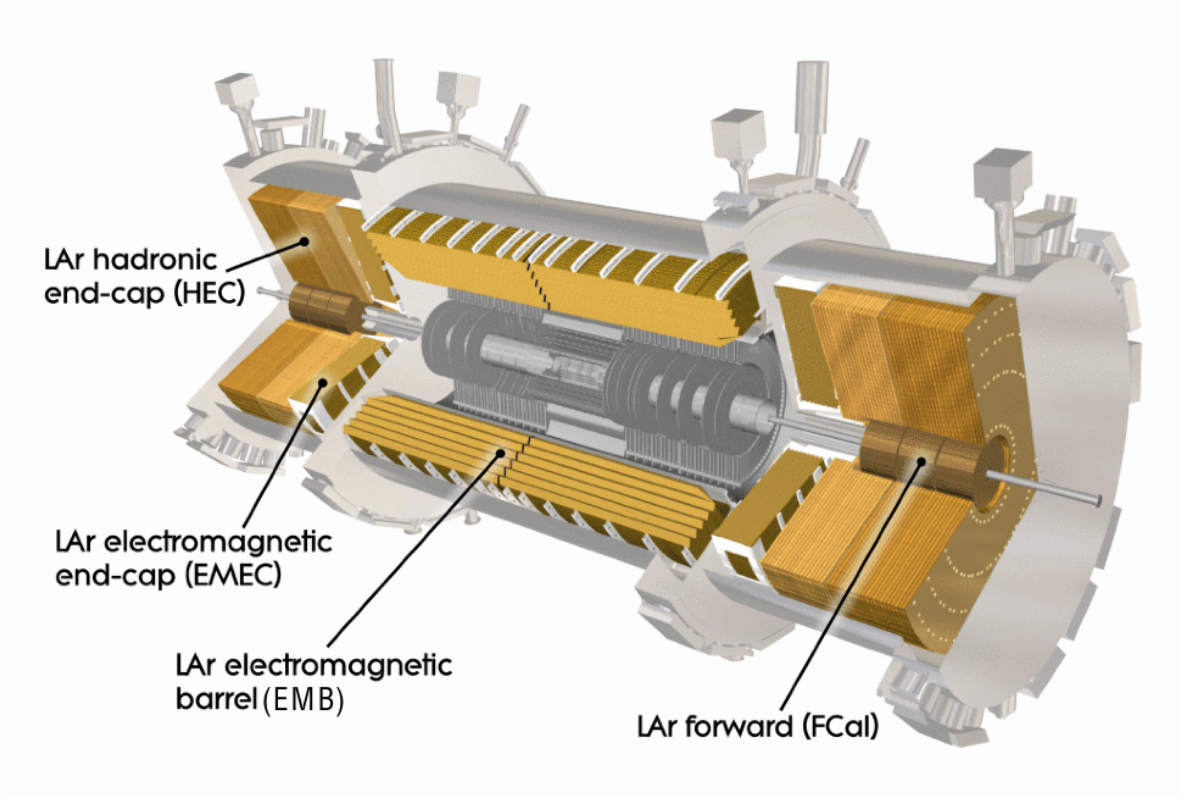
\includegraphics[width=0.8\linewidth]{atlas_cal.png}
    \caption{Схема калориметрической системы ATLAS}
    \label{fig:atlas_cal}
\end{figure}
Важной характеристикой системы калориметров является диапазон покрытия псевдобыстроты $|\eta|$. Эта величина показывает насколько направление движения элементарной частицы отличается от оси пучка и определяется как:
\begin{equation}
    \eta = -\ln(\tan(\frac{\Theta}{2})),
\end{equation}\par
где $\Theta$ -- угол между направлением импульса частицы и осью пучка. В физике коллайдеров зачастую используют именно этот показатель вместо простого полярного угла $\Theta$ в силу той особенности, что плотность числа рождённых частиц приблизительно постоянна в единицу $|\eta|$. По этой причине калориметры обычно сегментируют по псевдобыстроте, а не по телесному углу. Калориметрическая система ATLAS охватывает диапазон $|\eta|$ до 4.9.

\subsubsection{Электромагнитный калориметр}
Для прецизионного детектирования и измерения электронов и фотонов калориметрическая система ATLAS включает в себя электромагнитный калориметр. Он состоит из центрального (баррельного) блока (EMB -- electromagnetic barrel), покрывающего диапазон псевдобыстрот $|\eta| < 1,475$, и пары торцевых частей (EMEC -- electromagnetic end-cap), соответствующих области $1,375 < |\eta| < 3,2$. Электромагнитные калориметры ATLAS построены по гетерогенному принципу, то есть в них разделены функции поглощения и детектирования. В качестве активного вещества служит жидкий аргон, находящийся при температуре около 90K, а для поглощающего материала используется свинец. Между пластинами поглотителя также располагаются медно-каптоновые электроды, по которым происходит снятие сигнала.\par
Заряженная частица, попадая в калориметр, порождает в нём электромагнитный ливень (рис. \ref{fig:em_shower})\parencite{em_shower_wiki}, который детектируется по принципу ионизационной камеры: под воздействием электрического поля между заземлённым поглотителем и электродом, находящимся под высоким напряжением, ионы и электроны дрейфуют, причём последние индуцируют треугольный импульс на электроде(рис. \ref{fig:tri_impulse})(в действительности, сигнал является более сложным, чем просто треугольник -- в силу поглощения электронов загрязняющими примесями в активном веществе, такими как кислород или хлор, результирующий сигнал падает, а его форма домножается на небольшую экспоненту). Высота индуцированного импульса пропорциональна энергии, накопленной в ячейке калориметра. Время пика импульса используется для определения времени появления частицы.\par
\begin{figure}[ht]
    \centering
    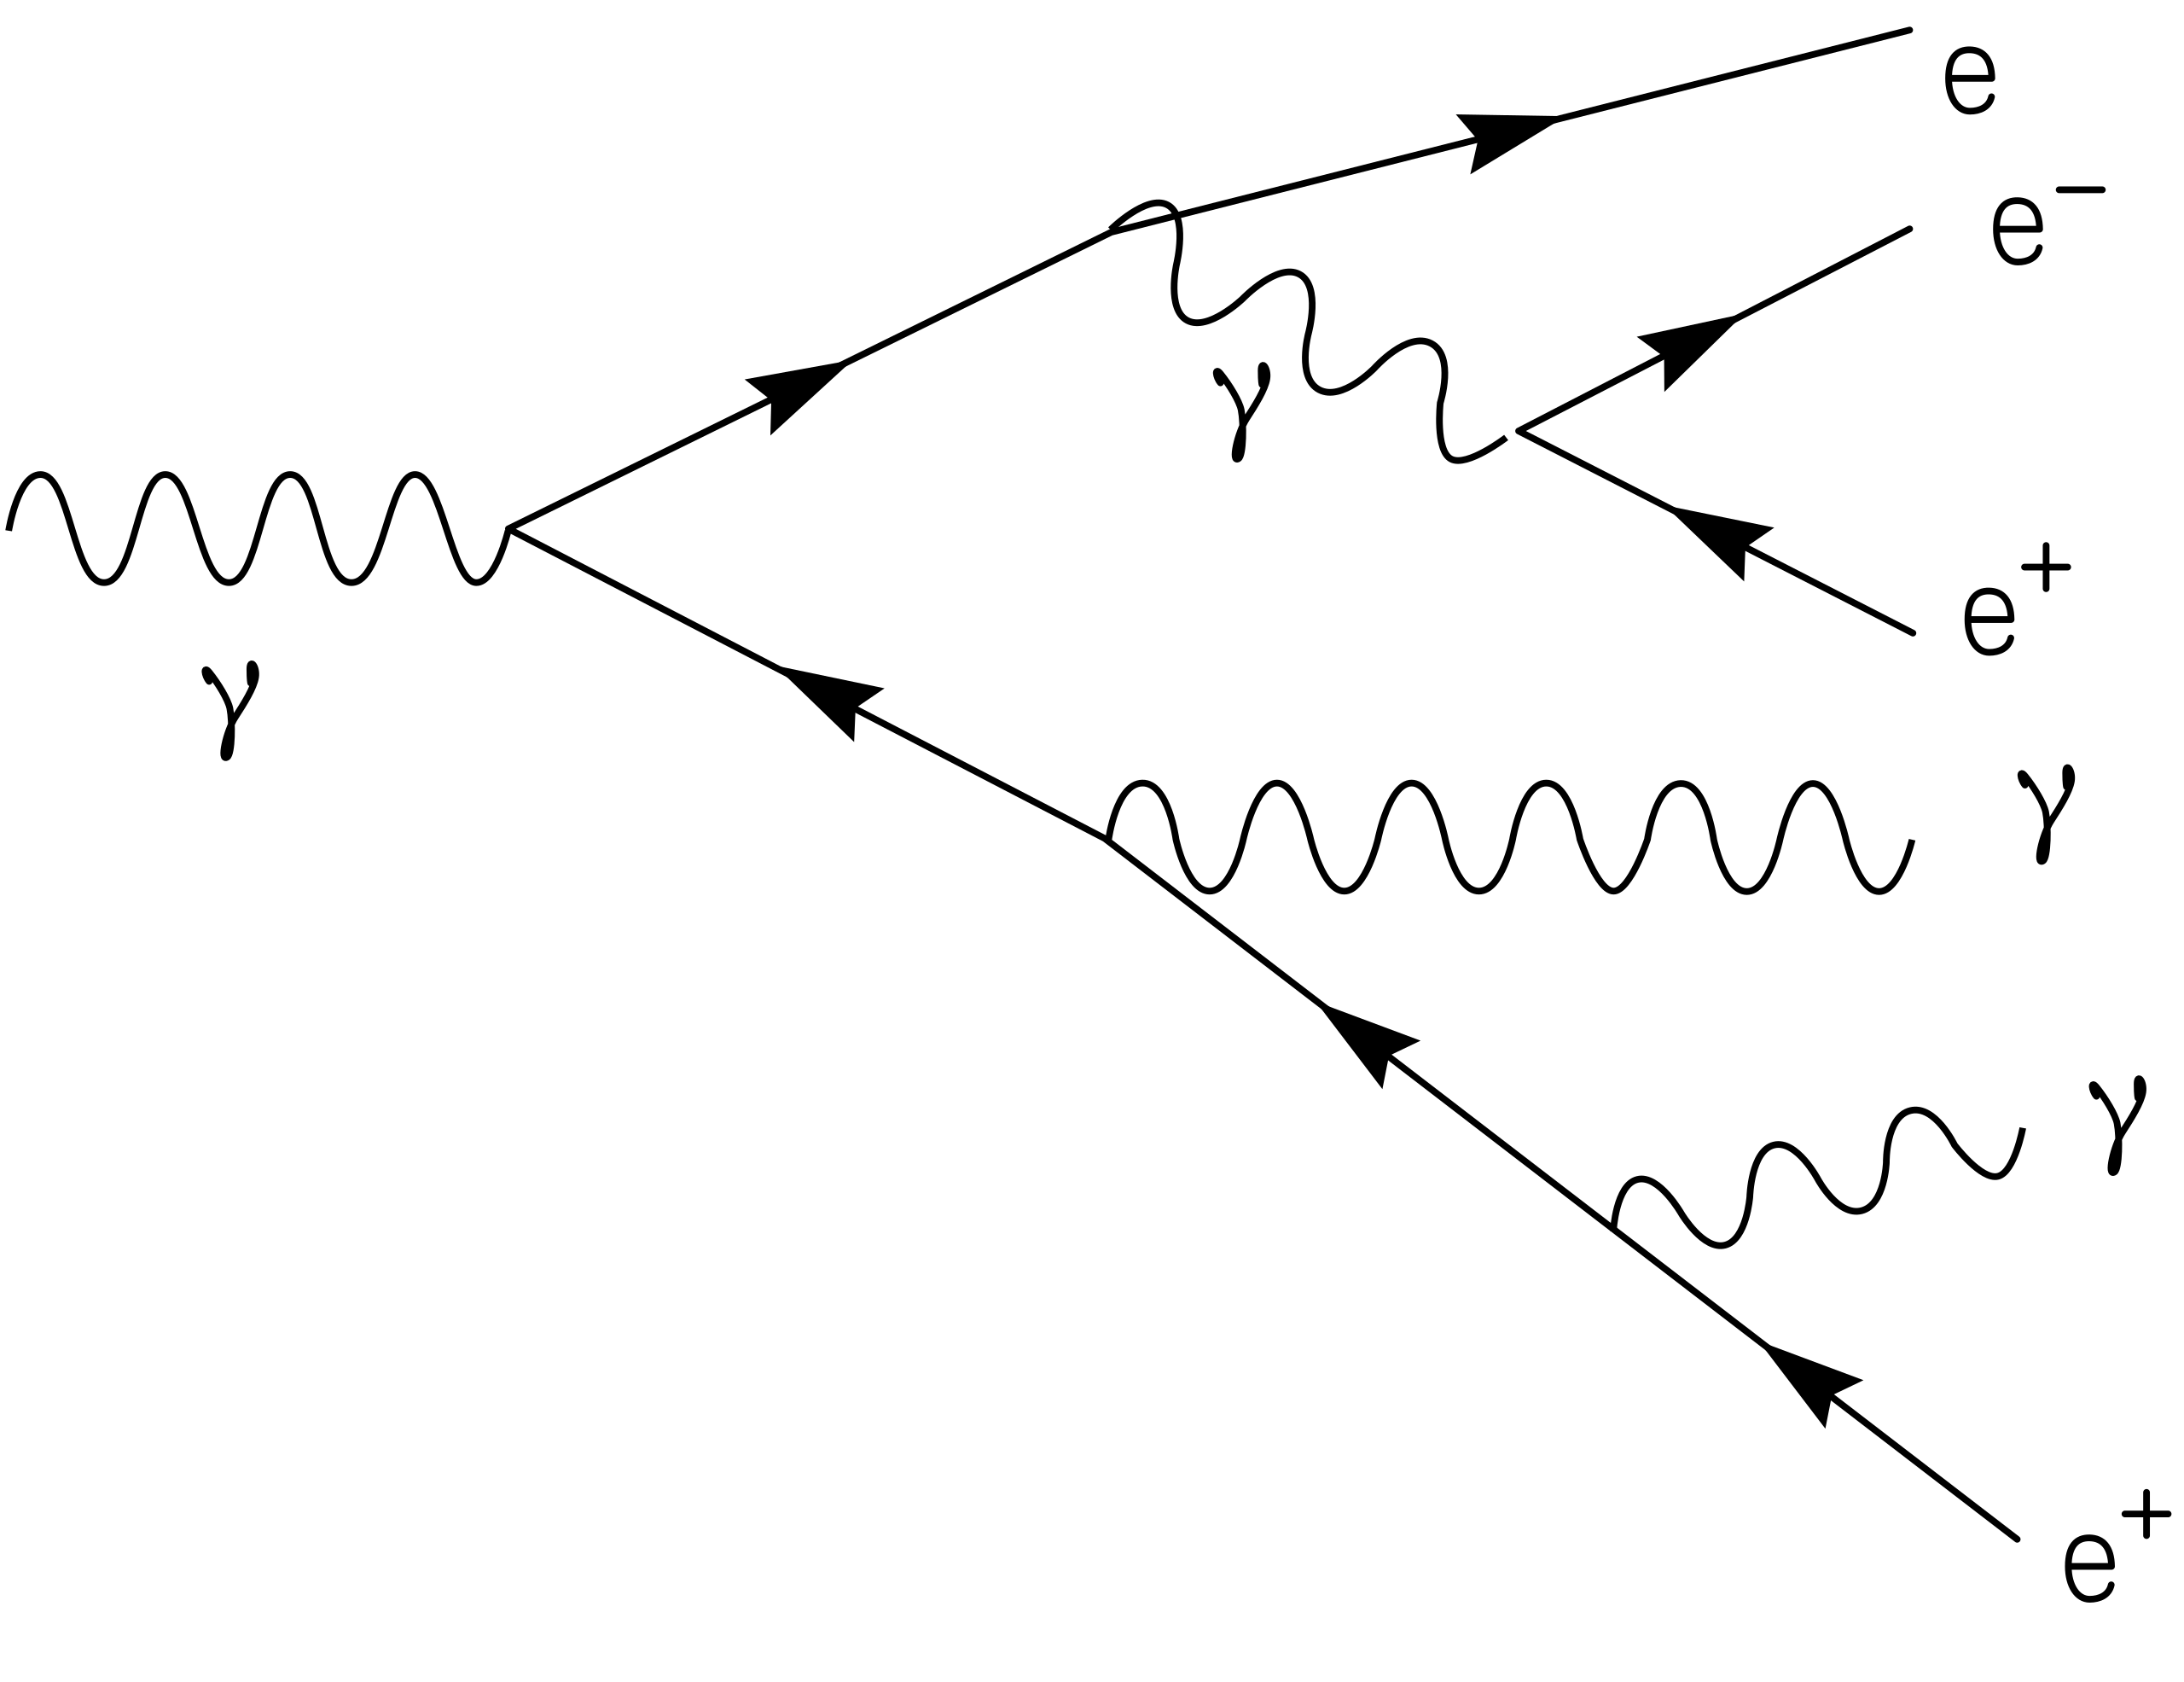
\includegraphics[width=0.5\linewidth]{em_shower.png}
    \caption{Схема электромагнитного ливня}
    \label{fig:em_shower}
\end{figure}
\begin{figure}[ht]
    \centering
    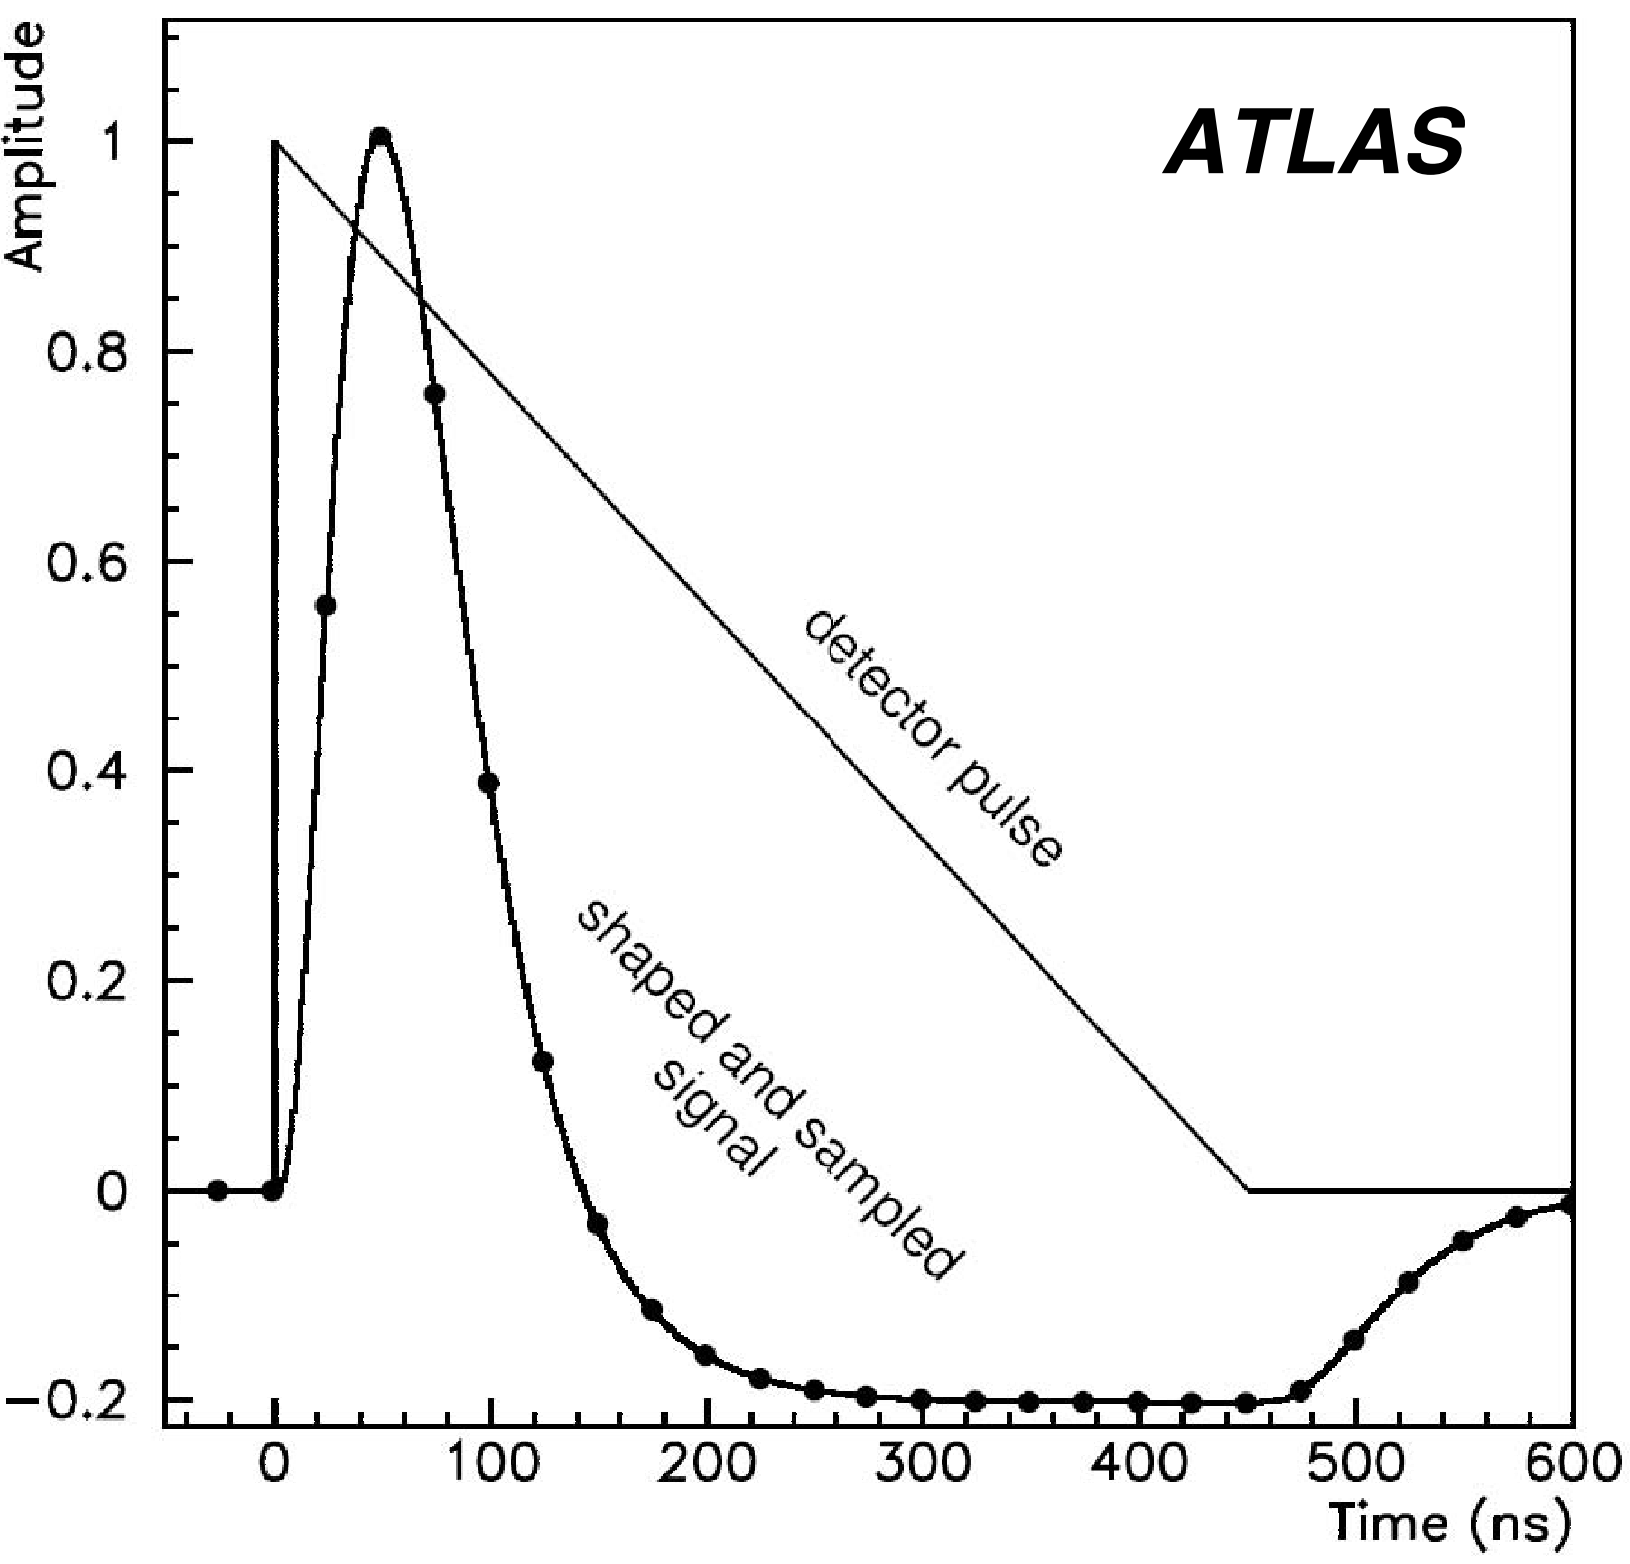
\includegraphics[width=0.5\linewidth]{tri_impulse.png}
    \caption{Форма импульса тока электромагнитного калориметра и выходного сигнала после формирования}
    \label{fig:tri_impulse}
\end{figure}
Электромагнитный калориметр имеет сложную геометрию в форме гармошки (аккордеон). Это позволяет достичь полной симметрии калориметра по азимутальному углу, а также обеспечить высокую гранулированность детектора и увеличить его быстродействие за счёт малого зазора между пластинами. Толщина EMB составляет более 24 радиационных длин ($X_0$, расстояние, на котором интенсивность потока электронов высокой энергии и гамма-излучения падает в e раз). Каждый модуль калориметра имеет ячеистую структуру и поделён на несколько слоёв по глубине, как, например, модуль центрального блока на рис. \ref{fig:em_cal_struct}. Калориметр сконструирован так, что наибольшая часть энергии собирается в среднем слое, задний слой собирает лишь хвост электромагнитного потока. Передний слой сегментирован таким образом, чтобы с его помощью можно было максимально точно определить направление падающих частиц. Исходя из этого, используя измерение энергии и положения всех ячеек в каждом слое калориметра можно восстановить энергию и траекторию рождённых частиц.
\begin{figure}[ht]
    \centering
    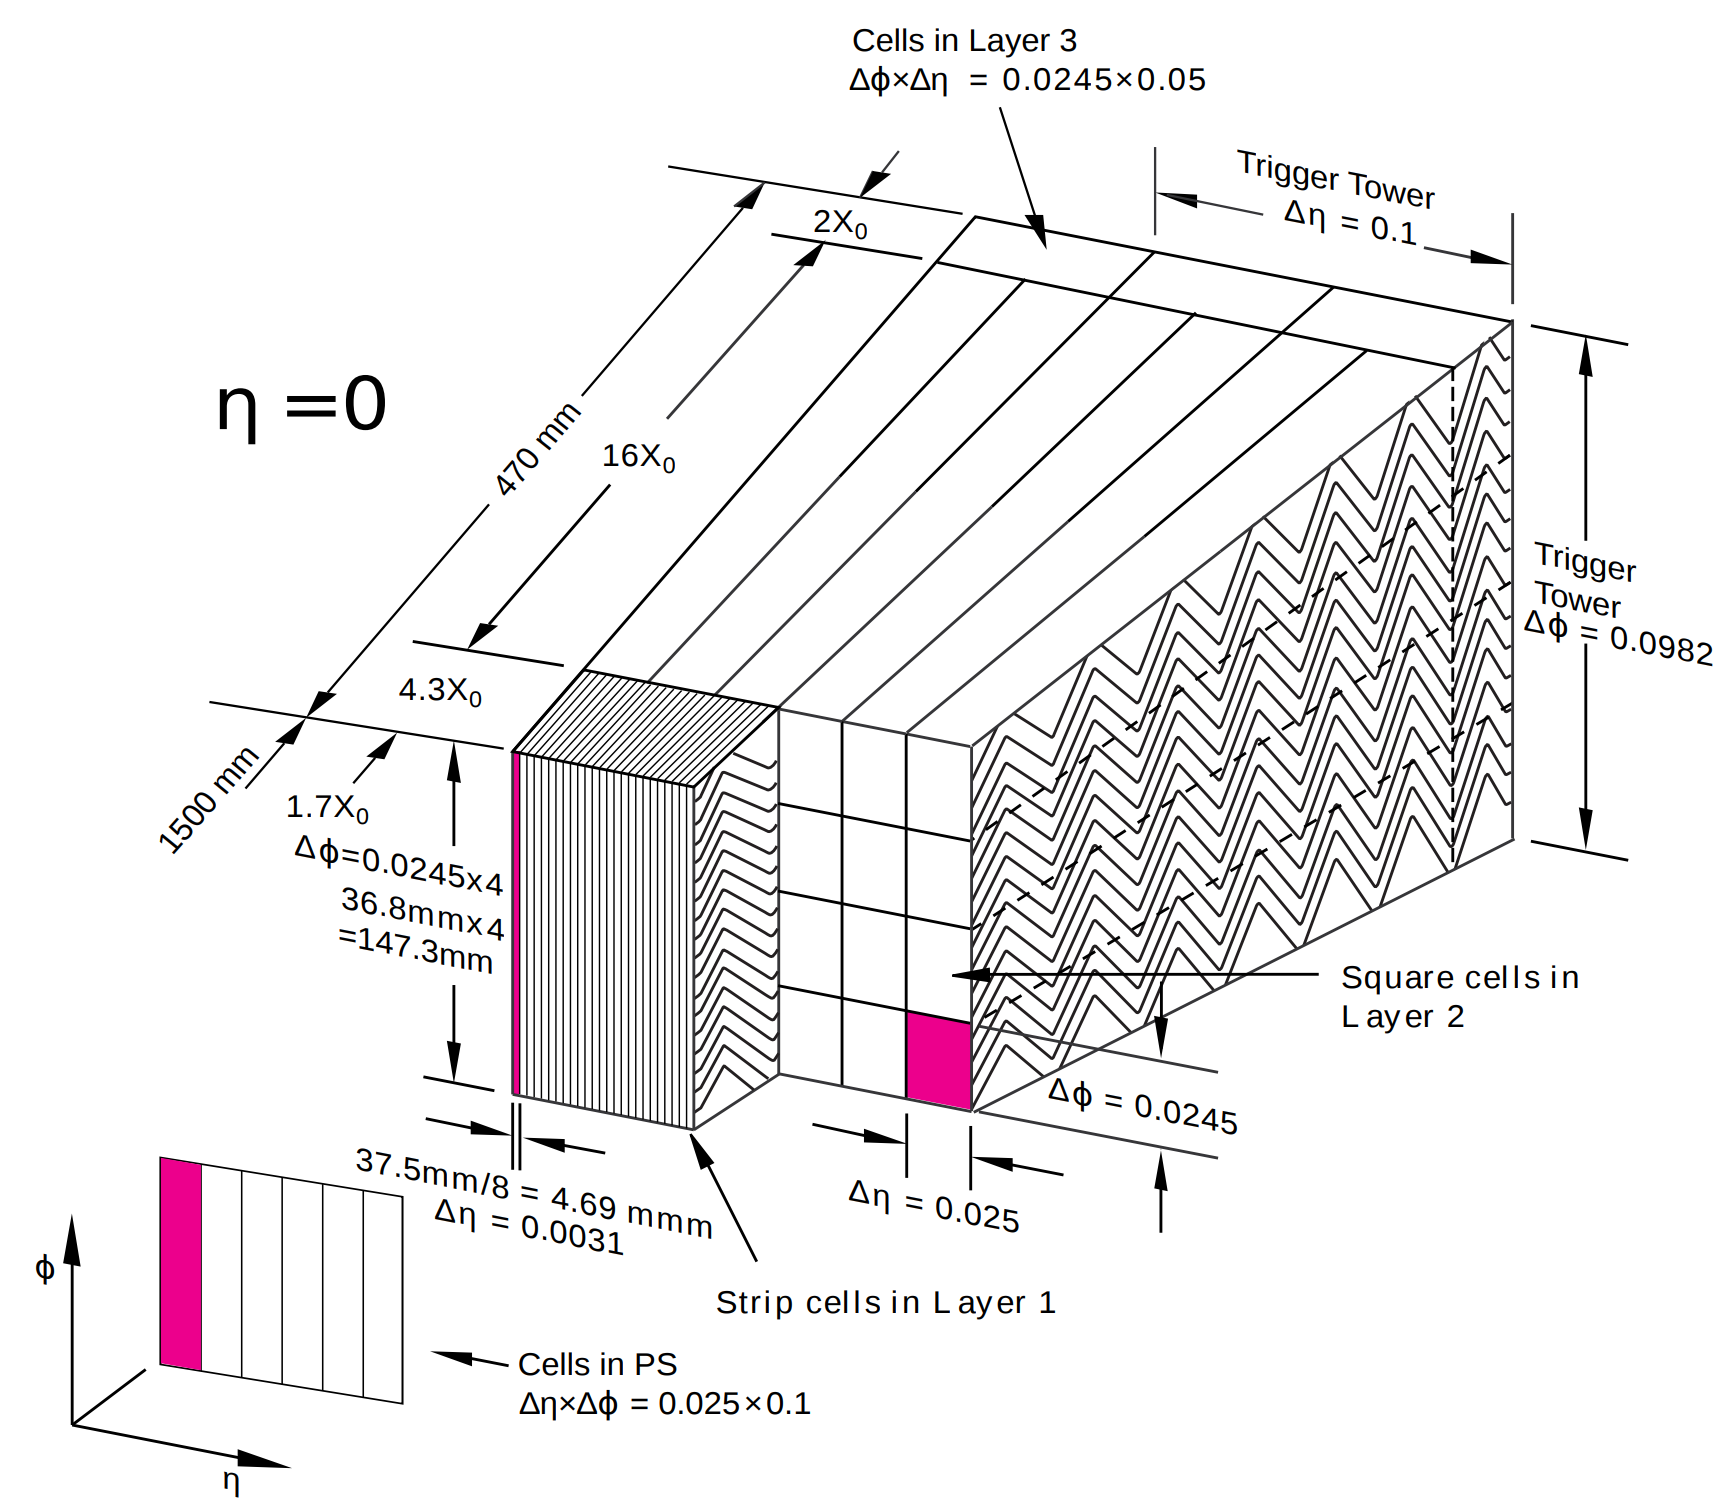
\includegraphics[width=0.7\linewidth]{em_cal_struct.png}
    \caption{Схема разделения модуля EMB по слоям}
    \label{fig:em_cal_struct}
\end{figure}


\subsubsection{Торцевой адронный калориметр}
Торцевой адронный калориметр(HEC -- hadronic end-cap) детектора ATLAS состоит из двух независимых колёс, которые установлены за блоками торцевого электромагнитного калориметра. Он обеспечивает адронное покрытие псевдобыстроты в диапазоне $1,5 < |\eta| < 3,2$. По принципу действия торцевой адронный калориметр похож на электромагнитный, но имеет плоскопараллельную структуру внутренней геометрии с медными пластинами-поглотителями, а в качестве адсорбера в нём используется железо.\par
Оба колеса калориметра состоят из 32 одинаковых по азимуту модулей. Переднее колесо разделено по глубине на две секции считывания, которые суммарно содержат 24 слоя поглотителя. Заднее колесо выполнено из 16 слоёв поглотителя, объединённых в один сегмент считывания. С каждой полученной ячейки регистрируется отдельный сигнал. Для обеспечения наилучшего отношения сигнала и шума предусилители считывающей электроники калориметра находятся в среде с низкой температурой и расположены по внешнему радиусу модулей.\par
Важным аспектом адронного калориметра является его способность обнаруживать мюоны, а также измерять их любые ионизационные потери и треки.\par


\subsubsection{Форвард калориметр}
Форвард калориметр находится ближе всего к пучку и обеспечивает электромагнитную и адронную калориметрию в диапазоне $3,2 < |\eta| < 4.9$. Из-за своего расположения он подвергается очень сильному воздействию дозы облучения мощностью до $10^6$ ${^\text{Гр}} / _\text{год}$ и потока нейтронов с кинетической энергией более 100 кэВ до 109 $\text{см}^{-2}\text{c}^{-1}$\parencite{tdr_old}. С учётом этих условий форвард калориметр разрабатывался с использованием следующих принципов:
\begin{itemize}
    \item механическая простота с применением небольшого набора материалов;
    \item использование радстойких материалов;
    \item использование материалов с высоким значением Z;
    \item достижение максимальной проективной толщины (вдоль проективных лучей от точки столкновения частиц);
    \item достижение максимальной средней плотности.
\end{itemize}\par
Калориметр состоит из трёх модулей: электромагнитного и двух адронных. В электромагнитной секции в качестве материала адсорбера используется медь, тогда как в адронных -- вольфрам. Номинальные внешние размеры у всех трёх модулей равные. Внутренняя структура представляет собой матрицу шестигранных трубок, расположенных вдоль пучка и изготовленных из материала поглотителя, в которые концентрично установлены медные электроды (рис. \ref{fig:f_cal_struct}). Пространство между стенками трубок и электродами заполнено жидким аргоном, выполняющим роль активного вещества. Конструкция позволяет точно контролировать зазор между электродами.
\begin{figure}[ht]
    \centering
    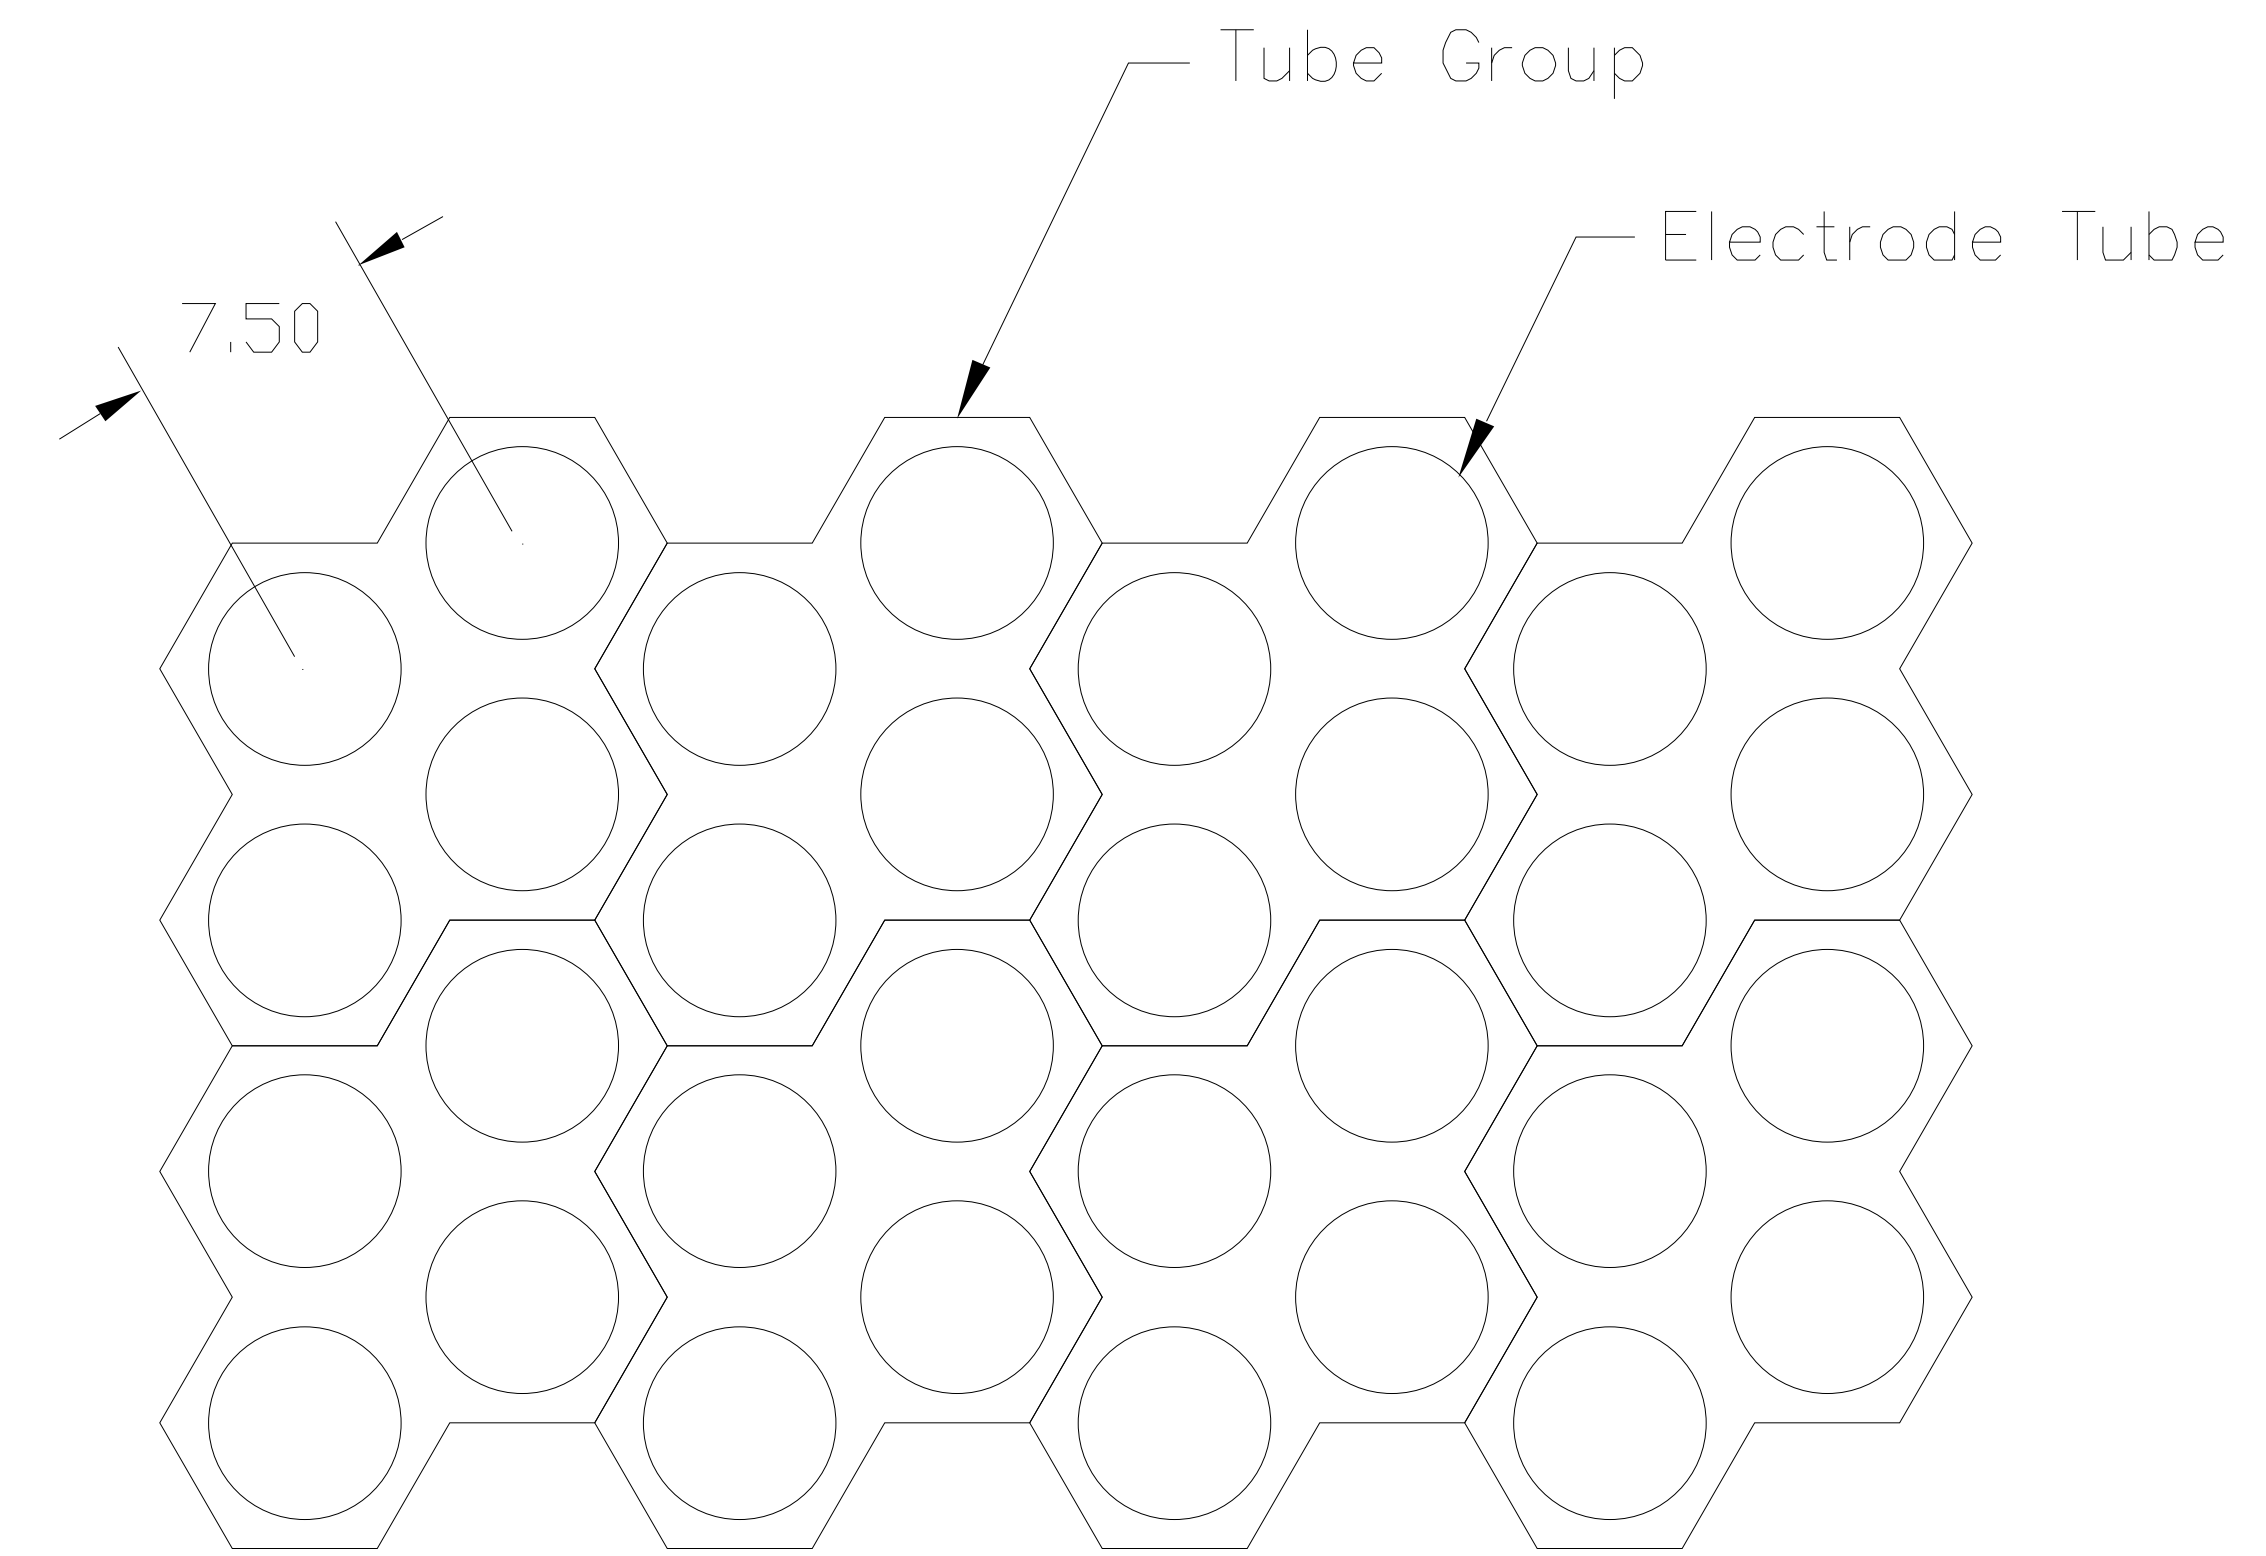
\includegraphics[width=0.6\linewidth]{f_cal_struct.png}
    \caption{Схема внутренней структуры форвард калориметра\parencite{tdr_old}}
    \label{fig:f_cal_struct}
\end{figure}\par
Таким образом, форвард калориметр способен работать в крайне радиационно нагруженных условиях, но при этом имеет сравнительно низкое разрешение. Однако, учитывая тот факт, что проходящие через него частицы имеют одни из наибольших абсолютных энергий, относительная точность остаётся достаточно высокой и такого разрешения вполне хватает для решения существующих физических задач.


\subsection{Считывающая электроника}
Считывающая электроника жидкаргоновых калориметров детектора ATLAS имеет сложную структуру, но в самом верхнем уровне её можно разделить на 2 части: фронтенд и задетекторную электронику. На рис. \ref{fig:read_electronics} изображена общая схема устройства считывающей электроники системы жидкоаргоновы калориметров.
\begin{figure}[ht]
    \centering
    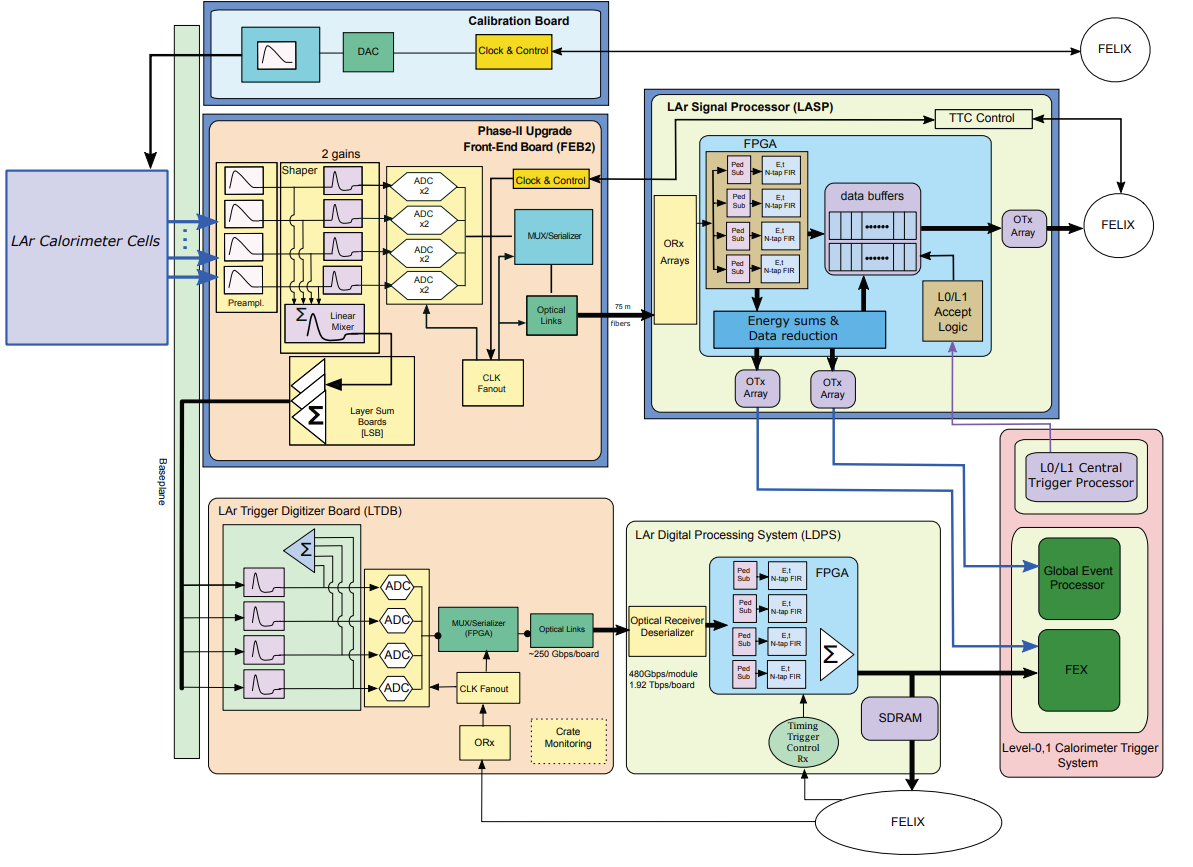
\includegraphics[width=\linewidth]{read_electronics.png}
    \caption{Схема считывающей электроники жидкоаргоновых калориметров ATLAS}
    \label{fig:read_electronics}
\end{figure}\par
Фронтенд часть располагается в непосредственной близости с ускорителем, поэтому на неё налагаются определённые требования по радиационной стойкости и отказоустойчивости. В рамках второй фазы обновления электроники на детектор будут установлены новые платы считывания FEB2(FEB -- Front-End Board), а также платы калибровки.\par

\subsubsection{Модуль FEB2}
Платы FEB2 принимают сигналы от калориметрических ячеек и выполняют их аналоговую обработку, включая усиление, формирование и разделение на две перекрывающиеся шкалы линейного усиления. Обе шкалы усиления оцифровываются при помощи аналого-цифрового преобразователя (АЦП), после чего цифровые сигналы сериализуются и отправляются через оптический канал связи. Для этого используется несколько специализированных интегральных микросхем, а также системы управления и синхронизации. Оцифровка данных производится на частоте 40 МГц, равной частоте столкновения частиц. Каждая плата FEB2 способна обрабатывать 128 калориметрических каналов, а для считывания всей системы жидкоаргоновых калориметров требуется 1524 таких устройства.\par
Аналоговая обработка данных выполняется в 2 этапа. На первом этапе выполняется усиление сигналов калориметра, которые имеют динамический диапазон до 16 бит, с помощью специального предусилителя. Второй каскад -- формирователь, который преследует две цели. Во-первых, он необходим для преобразования выходного сигнала схемы предварительного усилителя в дифференциальный выходной сигнал с несколькими коэффициентами усиления, а во-вторых, для получения по крайней мере одного этапа формирования в соответствии с требованиями к обработке сигнала. При необходимости могут быть добавлены несколько эквивалентных этапов формирования с минимальными затратами энергии. Как предусилитель, так и формирователь реализуются в одной специализированной интегральной микросхеме LAPAS (Liquid Argon Preamplifier And Shaper \parencite{lapas}), способной обрабатывать 4 либо 8 калориметрических сигналов.\par
В дополнение к усилению и формированию сигнала необходимы периферийные схемы, такие как генератор тестовых импульсов, схема смещения, датчик температуры, а также регистры конфигурации всего модуля.\par
Далее аналоговый сигнал от каждой калориметрической ячейки оцифровывается с частотой 40 МГц, синхронно с частотой соударения пучков в Большом Адронном коллайдере. Для охвата 16-битного динамического диапазона сигнал оцифровывается с двумя шкалами усиления с помощью 14-битных АЦП. Затем каждый выходной сигнал АЦП форматируется в 16-битное слово и сериализуется со скоростью передачи данных 640 Мбит/с. Каждое такое слово помимо 14 бит данных АЦП содержит бит чётности для обеспечения проверки ошибок. Учитывая, что каждая плата FEB2 обрабатывает 128 калориметрических каналов, результирующая скорость передачи данных составляет 163,84 Гбит/с (256 потоков по 640 Мбит/с каждый). Для передачи оцифрованных данных используются специально разработанные радиационно-стойкие трансивер и лазер lpGBT (low power GigaBit Tranceiver \parencite{lpgbt}). \par
Для реализации корректной синхронизации данных калориметра в модуле FEB2 предусмотрена генерация идентификатора соударения пучков (BCID -- Bunch Crossing Identifier). Данный идентификатор представлен в виде 12-битного счётчика, который инкриминируется с частотой возникновения событий в коллайдере и сбрасывается после каждого завершения цикла столкновений пучков частиц на орбите. Значение BCID, как и данные АЦП, сериализуются и передаются в систему задетекторной электроники через оптический канал.\par
Кроме основного тракта данных в модуле FEB2 присутствует подсистема, которая обеспечивает формирование входных данных для платы LTDB (LAr Trigger Digitizer Board \parencite{ltdb}). Данная плата обрабатывает аналоговые суммы сигналов для максимально быстрого принятия решения триггерной системы, но с более грубой детализацией, чем обеспечивается основным считыванием. Модуль FEB2 имеет набор сумматоров, которые формируют требуемые аналоговые сигналы сумм по соседним ячейкам калориметра.\par


\subsubsection{Модуль LTDB}
\input{sections/atlas_experiment/reading_electronics/ltdb.tex}

\subsubsection{Калибровочная система}
Важной частью фронтенд электроники является калибровочная система. С помощью специальных плат реализуется подача точных калибровочных сигналов непосредственно на ячейки жидкоаргонового калориметра. Форма калибровочного сигнала максимально приближена к импульсу ионизации, генерируемому электромагнитным ливнем в детекторе. В силу того, что получить истинно треугольный сигнал с помощью электронной схемы достаточно трудно, первоначально создаётся экспоненциальный импульс, у которого обрезается область затухания для максимального приближения к желаемой треугольной форме, по крайней мере, в начальной части импульса. Для компенсации остаточной разницы в форме между физическим импульсом ионизации и калибровочным сигналом производится непосредственное измерение свойств последнего для их учёта в процедуре калибровки.\par




    \newpage

\section{Сигнальный процессор жидкоаргонового калориметра (LASP)}
    Основным элементом задетекторной считывающей электроники жидкоаргонового калориметра детектора ATLAS в рамках второй фазы обновления являются модули сигнального процессора LASP (Liquid Argon Signal Processor). Они предназначены для принятия оцифрованных данных с модулей FEB2 и применения к ним цифровой фильтрации, их буферизации до появления сигнала триггера и последующей передачи в систему сбора данных DAQ. Также система LASP обеспечивает подготовку входныз данных для таких систем, как глобальный триггер и fFEX(forward Feature EXtractor). Система глобального триггера будет получать значения энергий только от тех ячеек, которые превышают заданный порог, определённый относительно общего шума. Таким образом, полосой пропускания данных можно управлять, сохраняя при этом достаточную количество информации для кластеризации событий.\par
Сигнальные процессоры рассчитаны на приём непрерывного потока оцифрованных данных с плат FEB2 на частоте соударения пучков частиц в Большом Адронном коллайдере (фактическая частота составляет 40.07897 МГц) для всех 182486 ячеек жидкоаргонового калориметра. Каждый модуль будет получать исходные данные с 8 плат FEB2, то есть с 1024 калориметрических ячеек. В настоящее время ведётся активная разработка этой системы.\par
Модули LASP требуют высокой пропускной способности ввода и вывода, а также возможности гибкого программирования алгоритмов обработки данных, цифровой фильтрации и сокращения объёма данных, поэтому в качестве основных вычислительных блоков LASP предусмотрены программируемые интегральные микросхемы. На плате каждого модуля будет располагаться 2 таких чипа для увеличения пропускной способности. Внутренняя структура дизайна программируемой логики представлена на рисунке \ref{fig:lasp}.

\begin{figure}[ht]
    \centering
    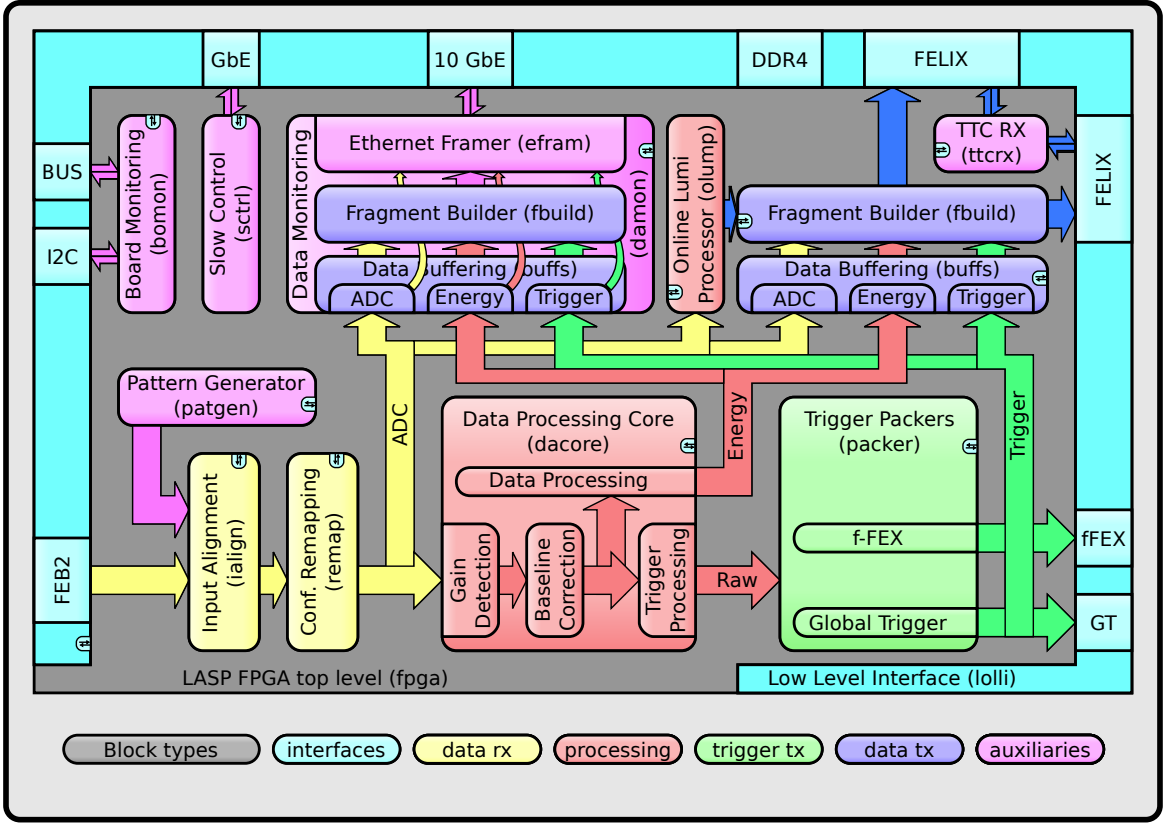
\includegraphics[width=\linewidth]{lasp.png}
    \caption{Блок схема прошивки LASP}
    \label{fig:lasp}
\end{figure}\par

Основными модулями сигнального процессора LASP являются:\par
\begin{itemize}
    \item интерфейс нижнего уровня lolli;
    \item система медленного контроля sctrl;
    \item генератор тестовых сигналов patgen;
    \item выравниватель входных данных ialign;
    \item модуль конфигурируемой перестановки remap;
    \item ядро обработки данных dacore;
    \item онлайн процессор светимости olump;
    \item упаковщик триггерных данных packer;
    \item блок буферов buffs;
    \item модуль форматирования данных fbuild;
    \item damon;
    \item монитор состояния аппаратуры bomon.
\end{itemize}\par

Для работы сигнального процессора используется целый набор различных тактовых сигналов. Среди основных можно выделить:
\begin{itemize}
    \item $f_{feb}$ -- тактовая частота, синхронно с которой поступают входные данные с системы FEB2. Имеет фиксированное значение 320 МГц;
    \item $f_{core}$ --  тактовая частота, синхронно с которой происходит непосредственная обработка данных. В зависимости от конфигурации может быть либо 320 МГц -- так называемая медленная опция, либо 480 МГц -- быстрая опция;
    \item $f_{sctrl}$ -- тактовая частота, на которой функционирует интерфейс медленного контроля. Непосредственное значение составляет 100 МГц.
    \item $f_{xgbe}$ -- тактовая частота, необходимая для приёма и отправки данных через 10 Гбит Ethernet порт(X Gigabit Ethernet). Является стендартной для такого порта и составляет 156,25 МГц.
\end{itemize}\par
Также в системе присутствует ещё несколько вспомогательных тактовых сигналов, необходимых для работы DDR4 интерфейса и TTC RX.\par
Базовым модулем системы LASP, с помощью которого осуществляется взаимодействие с внешним миром, является интерфейс нижнего уровня \textbf{lolli}. Данная подсистема содержит реализации всех необходимых низкоуровневых внешних интерфейсов:\par
\begin{itemize}
    \item FEB2;
    \item Gigabit Ethernet;
    \item 10 Gigabit Ethernet;
    \item DDR4 SDRAM;
    \item I2C;
    \item Custom BUS;
    \item fFEX;
    \item FELIX;
    \item Global Trigger.
\end{itemize}\par
При возможности, все интерфейсы из lolli в программируемую логику спроектированы с использованием стандартных потокового интерфейса Avalon Stream (AVST) и интерфейса, отображаемого на память Avalon Memory Mapped (AVMM). Это позволяет иметь четко определённые и документированные стандартные интерфейсы между каждым компонентом LASP.\par
Для реализации возможности управления всеми компонентами сигнального процессора, а также их соединения с внешним миром предусмотрена система медленного контроля \textbf{sctrl}. Она позволяет пользователю загружать или изменять все доступные пользователю параметры конфигурации, а также иметь доступ ко всем регистрам мониторинга и состояния любого модуля в режиме реального времени.\par
Компонент sctrl использует внешний канал связи Gigabit Ethernet, реализованный в интерфейсе lolli. Для общения с внутренними модулями используется AVMM интерфейс. Специально для интерфейса медленного контроля каждый модуль имеет набор выделенных регистров, в которых хранятся либо какие-нибудь параметры, либо данные о состоянии или некоторая статистика. Между этими регистрами есть глобальное разделение адресного пространства, через которое sctrl и способно доступаться к конкретным модулям.\par
В целях отладки системы в общей структуре релизован генератор тестовых данных \textbf{patgen}. С его помощью можно осуществлять ввод определяемых пользователем значений АЦП для обработки вместо данных, поступающих от FEB2. Такая возможность используется для тестирования системы и проверки основного функционала независимо от реальных данных с FEB2. Для корректной отладки с помощью pathen в него заложены следующие свойства:\par
\begin{itemize}
    \item данные, генерируемые patgen имеют ту же структуру, что и данные из FEB2;
    \item patgen способен иммитировать рассинхронизацию между каналами данных(сдвиг по идентификатору пучка);
    \item каждый канал имеет независмый источник данных;
    \item имеется возможность выбирать между двумя возможными источниками данных(patgen или FEB2) для каждого канала данных в отдельности;
    \item данные генерируются непрерывно циклическим образом, повторение происходит синхронизованно с циклом пучков на орбите.
\end{itemize}\par
Для снижения влияния на процесс компиляции системы целиком в проектирование генератор тестовых сигналов заложен принцип минимизации занимаемых логических ресурсов. В следствие этого, patgen имеет две версии реализации:\par
\begin{itemize}
    \item на основе оперативной памяти: в этой версии используются данные, хранимые во внутренней операвтивной памяти ПЛИС, записанные через интерфейс медленного контроля. Такой подход даёт большую гибкость, но занимает большой объём памяти;
    \item на основе функции генерации: в этой версии данные генерируются на лету, используя определённый алгоритм.
\end{itemize}\par
Первым модулем, который непосредственно принимает входные данные, является \textbf{ialign}. Он предназначен для осуществления выравнивания по времени поступающей информации с FEB2. Входной поток организован в виде кадров, содержащих данные АЦП и два идентификатора столкновения пучков для соответствующих шкал усиления, которые могут быть как идентичными, так и различными. В ходе обработки все данные АЦП выравниваются по одинаковому BCID. При этом порядок оцифрованных значений в рамках каждого отдельного канала может изменяться, однако он не предопределён заранее -- его можно настраивать индивидуально для любого потока, но идентично для парных значений по шкалам усиления.\par
Важная особенность обработки данных модулем ialign -- это расширение данных по временным ячейкам. То есть, по всем каналам с низкого уровня поступает по 6 значений АЦП для каждого идентификатора столкновения пучков, но данный модуль добавляет везде по 2 дополнительных невалидных значения, тем самым увеличивая число временных ячеек с данными АЦП до 8. На рисунке \ref{fig:ialign_output} схематично изображён выходной интерфейс компонента. Рабочей тактовой частотой для ialign является $f_{feb}$, соответствующая поступающим с FEB2 данным.

\begin{figure}[ht]
    \centering
    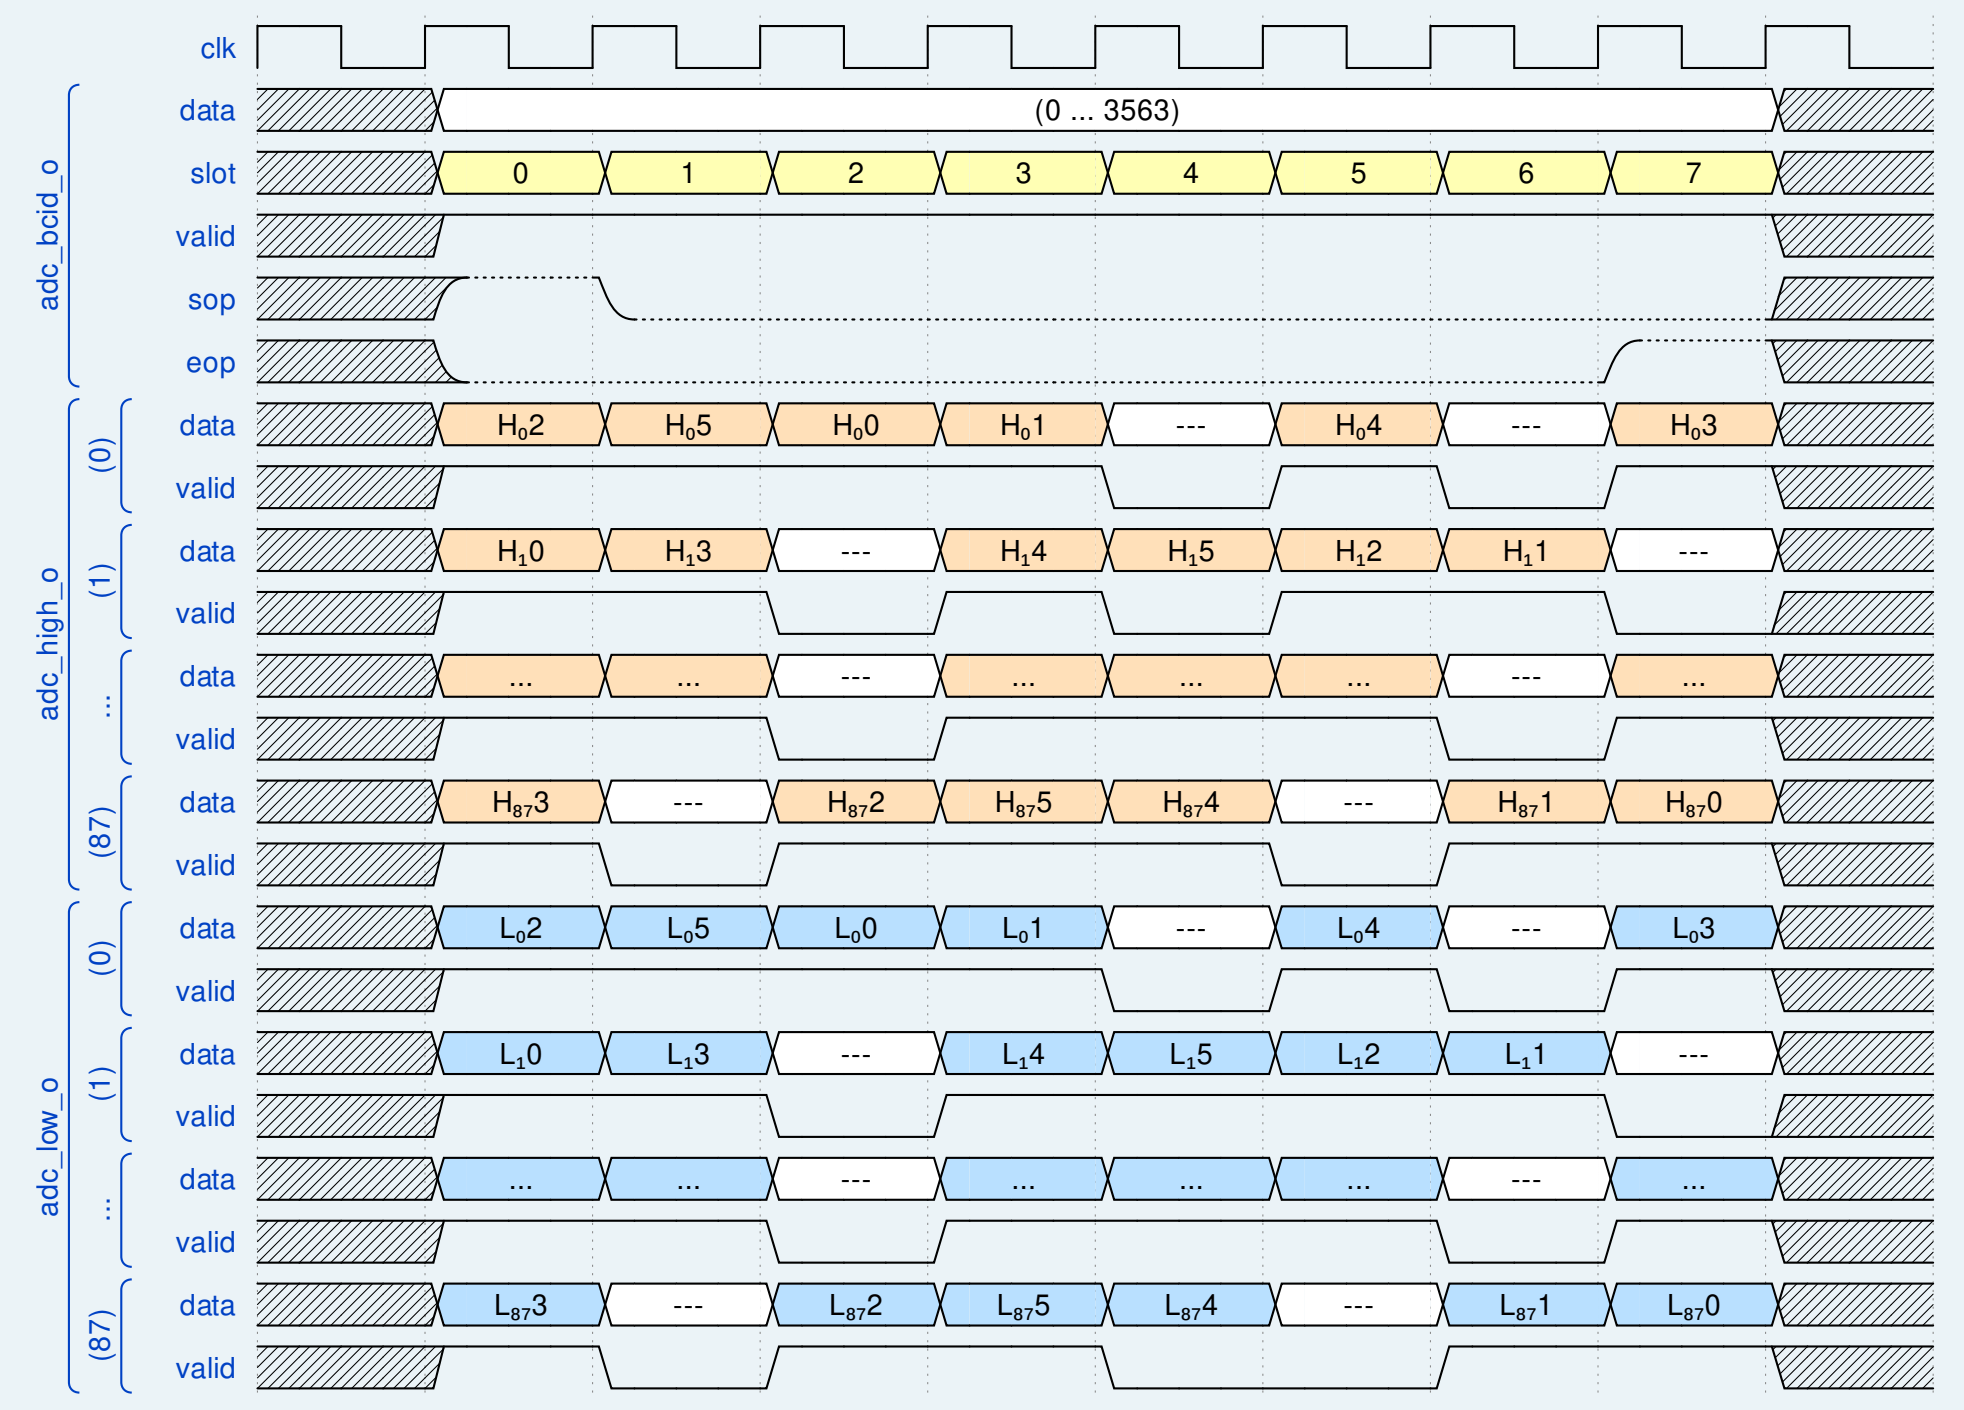
\includegraphics[width=\linewidth]{ialign_output.png}
    \caption{Выходной интерфейс модуля ialign}
    \label{fig:ialign_output}
\end{figure}\par

Следующий элемент тракта данных жидкоаргонового сигнального процессора LASP -- модуль \textbf{remap}. Он служит для изменения порядка данных в соответствии с геометрией детектора, ведь в силу ряда технических ограничений, информация от калориметрических ячеек, поступающая через FEB2, находится в перемешанном виде. Путём переупорядочивания данных упрощается задача вычисления сумм энергии ячеек жидкоаргонового калориметра. Такие суммы необходимы для уменьшения полосы пропускания данных в системе fFEX. Как и в случае модуля ialign схема перестановки не является предопределённой -- каждый выходной канал может быть гибко сконфигурирован согласно требованиям. Важной особенностью является то, что помимо всего прочего, компонент конфигурируемой перестановки необходим для реализации перехода данных из тактового домена $f_{feb}$ в домен сигнала $f_{core}$.\par
Сигнальный процессор LASP может иметь одну из двух конфигураций, так называемые медленную и быструю опции. В случае медленной опции remap принимает входной поток данных, состоящий из 88 каналов, в которых содержится по 8 значений АЦП для каждого идентификатора соударения пучка и преобразовывыет его в аналогичный поток, но имеющий лишь 64 точно таких же канала. При этом тактовые частоты $f_{feb}$ и $f_{core}$ совпадают по величине 320 МГц, однако могут быть сдвинутыми по фазе. Реальный объём полезных данных не уменьшается, как это может показаться на первый взгяд, поскольку четверть входного трафика составляют невалидные значения, добавленные модулем ialign, а также присутствуют сигналы, поступающие с неподключнных разъёмов FEB2. В конфигурации быстрой опции та же структура входных данных преобразовывается в 43 выходных канала, каждый из которых имеет целых 12 оцифрованных величин. Поскольку в любом варианте интервал между соседними моментами соударения пучков не изменяется и составляет 25 наносекунд, то в таком режиме тактовая частота выходной шины $f_{core}$ пропорционально увеличена и составляет 480 МГц для обеспечения необходимой плотности данных во времени.\par
Основным обрабатывающим компонентом процессора LASP является ядро обработки данных \textbf{dacore}. Оно преобразовывает поступающие от модуля конфигурируемой перестановки исходные значения АЦП в соответствующие энергетические величины с помощью специальных алгоритмов. Задачи обработки можно разделить на четыре основных функции:\par
\begin{itemize}
    \item определение оптимального коэффициента усиления;
    \item коррекция пъедистала;
    \item вычисление энергии, временной характеристики, а также параметра качества с оптимальным разрешением для системы хранения данных (однако вычисление параметра качества и временной характеристики выполняется только для калориметрических ячеек с выделившейся в них энергией выше заданного порога);
    \item вычисление энергии с уменьшенным разрешением для триггерной системы.
\end{itemize}\par
Следовательно, компонент dacore обеспечивает 2 отдельных выходных потока:\par
\begin{enumerate}
    \item поток для модуля упаковки данных packer, который содержит грубые энергетические значения и флаги превышения порога;
    \item поток для блока буферов, содержащий для каждой калориметрической ячейки энергетическоt значениt, бит оптимального коэффициента усиления и флаг превышения порога. Для высокоэнергетических ячеек добавляется время импульса и значение качества импульса.
\end{enumerate}\par
Для повышения точности данных, направляемых в систему хранения, используется дополнительная стадия обработки, реализующая алгоритмы цифровой фильтрации. С их помощью достигается восстановление энергии с точностью 1 МэВ, которая затем кодируется многолинейным способом.Для триггерных данных также предусмотрена цифровая фильтрация, предназначенная для подавления шумов и вычисление значений энергии с достаточной точностью для всех модулей принятия триггерных решений, подключенных к задетекторной электронике. Также для этих данных формируется по три бита превышения порогов, количественно описывающие переполнения фонового уровня энергии.\par
Одним из важнейших показателей работы коллайдера является светимость. Для его рассчёта в системе жидкоаргонового сигнального процессора предусмотрен модуль онлайн процессора светимости \textbf{olump}. Этот компонент усредняет необработанные оцифрованные значения АЦП, получаемые напрямую с модуля конфигурируемой перестановки remap, по каждому столкновению частиц. Его задачи можно разделить на 4 основных части:\par
\begin{enumerate}
    \item вычисление суммы и суммы квадратов измерений АЦП по шкале высокого коэффициента усиления для настраиваемого набора из 8 каналов. Эти величины вычисляются для каждого столкновения пучков и накапливаются по каждому набору;
    \item буферизация данных АЦП по шкале высокого коэффициента усиления в течение одного полного оборота пучков на орбите Большого Адронного коллайдера. Производится это по тем же наборам каналов, которые были определены выше;
    \item вычисление оценки мгновенной светимости для этих же подмножеств каналов. Эта оценка может быть использована в ядре обработки данных dacore для компенсации влияния светимости на восстановление энергетических и временных величин;
    \item сжатие без потерь значений сумм и сумм квадратов оцифрованных сигналов АЦП.
\end{enumerate}\par
Подготовка энергетических значений для их последующей передачи в триггерные системы задетекторной электроники осуществляется силами упаковщика триггерных данных \textbf{packer}. Задачи этого компонента заключаются в следующем:\par
\begin{itemize}
    \item группировка данных, полученных с ядра обработки данных;
    \item кодирование энергий с использованием многолинейного кодирования и их передача в системы глобального триггера и fFEX;
    \item отправка данных в блок буфферов;
    \item отправка данных в модуль damon.
\end{itemize}\par
Поток выходных данных для систем глобального триггера и fFEX состоит из кадров, которые содержат информацию о текущем соударении пучков. Помимо этого, в выходном канале требуется отправка служебных кадров, которые не содержат непосредственно полезные данные, а несут различную идентификационную информацию, необходимую, например, для синхронизации.\par
После обработки данные не сразу отправляются в систему хранения, а некоторое время ожидают соответствующего им триггерного сигнала в блоке буферов \textbf{buffs}. Буферизации подлежат все имеющиеся данные: изначальные значения АЦП, обработанные энергетические величины и триггерные данные, полученные от компонентов конфигурируемой перестановки remap, ядра обработки dacore и упаковщика packer соответственно. Время хранения информации требуется не меньшее, чем задержка триггера, которая составляет около 10 мкс.\par
Последний этап обработки данных -- формирование из готовых значений фрагментов, пригодных к отправке в FELIX через интерфейс нижнего уровня lolli. Эта задача выполняется с помощью модуля форматирования данных \textbf{fbuild}. Генерируемый формат данных может варьироваться в зависимости от назначения:\par
\begin{itemize}
    \item сбор данных;
    \item калибровка;
    \item отладка;
    \item тестирование системы;
    \item ввод в эксплуатацию.
\end{itemize}\par
Данные, содержащиеся во фрагментах, представляют собой исходные данные АЦП или энергетические значения и связанные с ними биты валидности и качества, а также данные, отправляемые в системы глобального триггера и fFEX. Формат кадра может потребовать отправки определённых или всех этих типов данных. Кроме того, можно выбирать один или несколько потоков выходных данных, хотя обычно используются все.\par
Кроме системы хранения данных результаты обработки могут передаваться на модуль мониторинга данных \textbf{damon}. Он обеспечивает низкоскоростной канал мониторинга исходных, обработанных и триггерных данных. Эти собранные значения буферизируются до тех пор, пока не будет принято решение о тои, отправлять ли их для мониторинга или нет. В конечном итоге, отобранная информация форматируется в Ethernet кадры, которые отправляются на порт XGbE интерфейса нижнего уровня lolli. Компонент damon предполагает реализацию двух возможных режимов работы:\par
\begin{enumerate}
    \item режим мониторинга: в этом режиме осуществляется полный сбор всех входящих данных всех ячеек, которые передаются лишь по определённому условию, например, получению сигнала триггера. Частота передачи этой информации ограничена пропускной способностью внешнего интерфейса(XGbE);
    \item режим прямой трансляции: в этом режиме производится непрерывные сбор и отправка всех входных данных, но лишь для небольшого числа ячеек. Ячейки, которые транслируются в текущий момент, определяются конфигурацией. Количество ячеек, участвующих в режиме трансляции ограничено пропускной способностью внешнего интерфейса(XGbE).
\end{enumerate}\par
Отдельным модулем, который не является частью тракта обработки данных жидкоаргоновых калориметров детектора ATLAS, однако имеет очень важное значение в функционировании жидкоаргонового сигнального процессора LASP можно выделить монитор состояния платы \textbf{bomon}. Модуль взаимодействует с устройствами, подключенным к ПЛИС через интерфейс I2C и микросхемой контроллера управления платформой IPMC (Intelligent Platform Management Controller). Bomon собирает и передаёт информацию о состоянии внутреннего оборудования ПЛИС LASP, такую как температуру, токи и напряжения, а также считываеь информацию с каждого из подключенных электрооптических модулей.\par

    \newpage

\section{Цель и задачи работы}
%    Главной целью данной работы является разработка блока упаковки данных для системы FEX модуля сигнального процессора LASP жидкоаргонового калориметра детектора ATLAS. Эта подсистема состоит из пары связки компонентов, а именно упаковщика данных packer для системы fFEX и  модуля конфигурируемой перестановки remap. То есть по каждому из компонентов необходимо проработать их внутреннюю архитектуру, после чего реализовать на языке описания цифровой логики, что также подразумевает под собой:\par
\begin{itemize}
    \item написание синтезируемых блоков логической аппаратуры;
    \item создание симуляционного окружения и отладка разработанной структуры;
    \item компиляция модулей под целевую платформу;
    \item проверка и оптимизация занимаемых логических ресурсов и временных задержек.
\end{itemize}\par
Помимо работы по непосредственной реализации указанных компонентов сигнального процессора LASP необходимо разработать:\par
\begin{itemize}
    \item программное обеспечение для автоматической генерации конфигураций модуля remap;
    \item формат кадра протокола передачи данных из модуля packer сигнального процессора LASP в систему fFEX.
\end{itemize}\par
В рамках проекта LASP коллаборации ATLAS принято использовать для работы язык описания аппаратуры VHDL. В качестве наиболее возможной потенциальной микросхемы ПЛИС на данный момент рассматривается кристаллы от компании Intel, принадлежащие высокопроизводительному семейству Stratix, а именно Intel Stratix 10 SX 1SX280HU1F50E2VG, являющийся системой на кристалле, имеющей наряду с программируемой логикой также производительный процессор ARM A53 или Intel Stratix 10 MX 1SM21BHU1F53E2VG. Поскольку целевым устройством в любом случае является продукция Intel, то, соответственно, в качестве инструмента разработки ключевую роль занимает программное обеспечение Intel Quartus Prime. Также, в рамках данного проекта применяется симулятор цифровых логических схем QuestaSim.\par

    \newpage

\section{Модуль конфигурируемой перестановки (Remap)}
    Модуль Remap является частью жидкоаргонового сигнального процессора LASP (рис. \ref{fig:remap_lasp}) и в первую очередь предназначен для организации упорядочивания входных данных в соответствии с геометрией детектора.\par
\begin{figure}[ht]
    \centering
    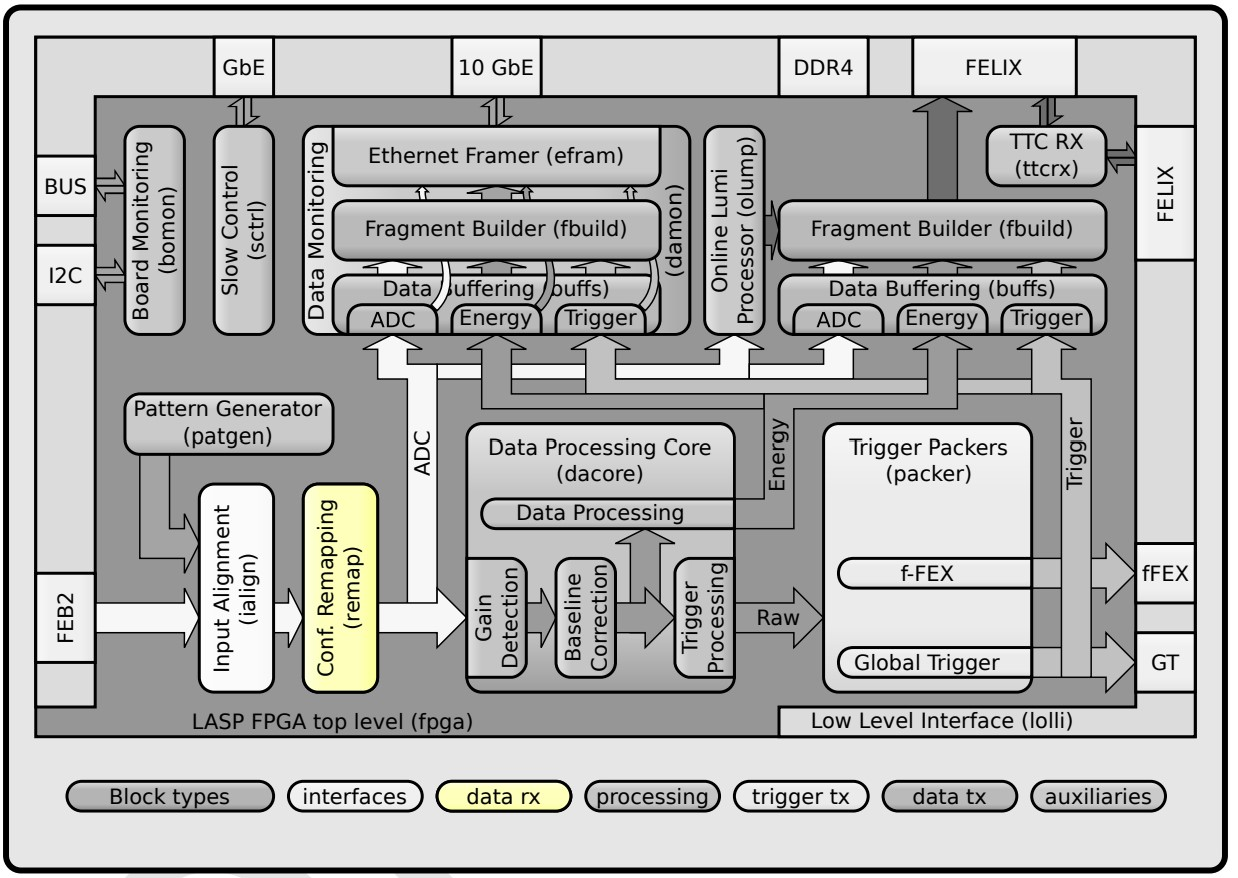
\includegraphics[width=0.8\linewidth]{remap_lasp.png}
    \caption{Схема расположения модуля Remap в общей структуре сигнального процессора LASP}
    \label{fig:remap_lasp}
\end{figure}\par
Remap компонент должен реализовывать приём поступающей информации и формировать из неё набор выходных каналов данных, в каждом из которых обязаны передаваться значения АЦП, выбранные из входных каналов в соответствии с установленной конфигурацией, в определённом порядке, также согласно конфигурации.\par

\subsection{Архитектура модуля}
Основополагающим подходом в проектировании модуля конфигурируемой перестановки \texttt{remap} является создание таких элементарных устройств, которые способны принимать на вход весь требуемый объём данных и формировать из него лишь один выходной канал. Это обеспечивает высокую гибкость в масштабировании, поскольку в таком случае реализация необходимого количества выходных каналов достигается простой репликацией подобных структур, как это показано на рисунке \ref{fig:remap_replication}.\par

\begin{figure}[ht]
    \centering
    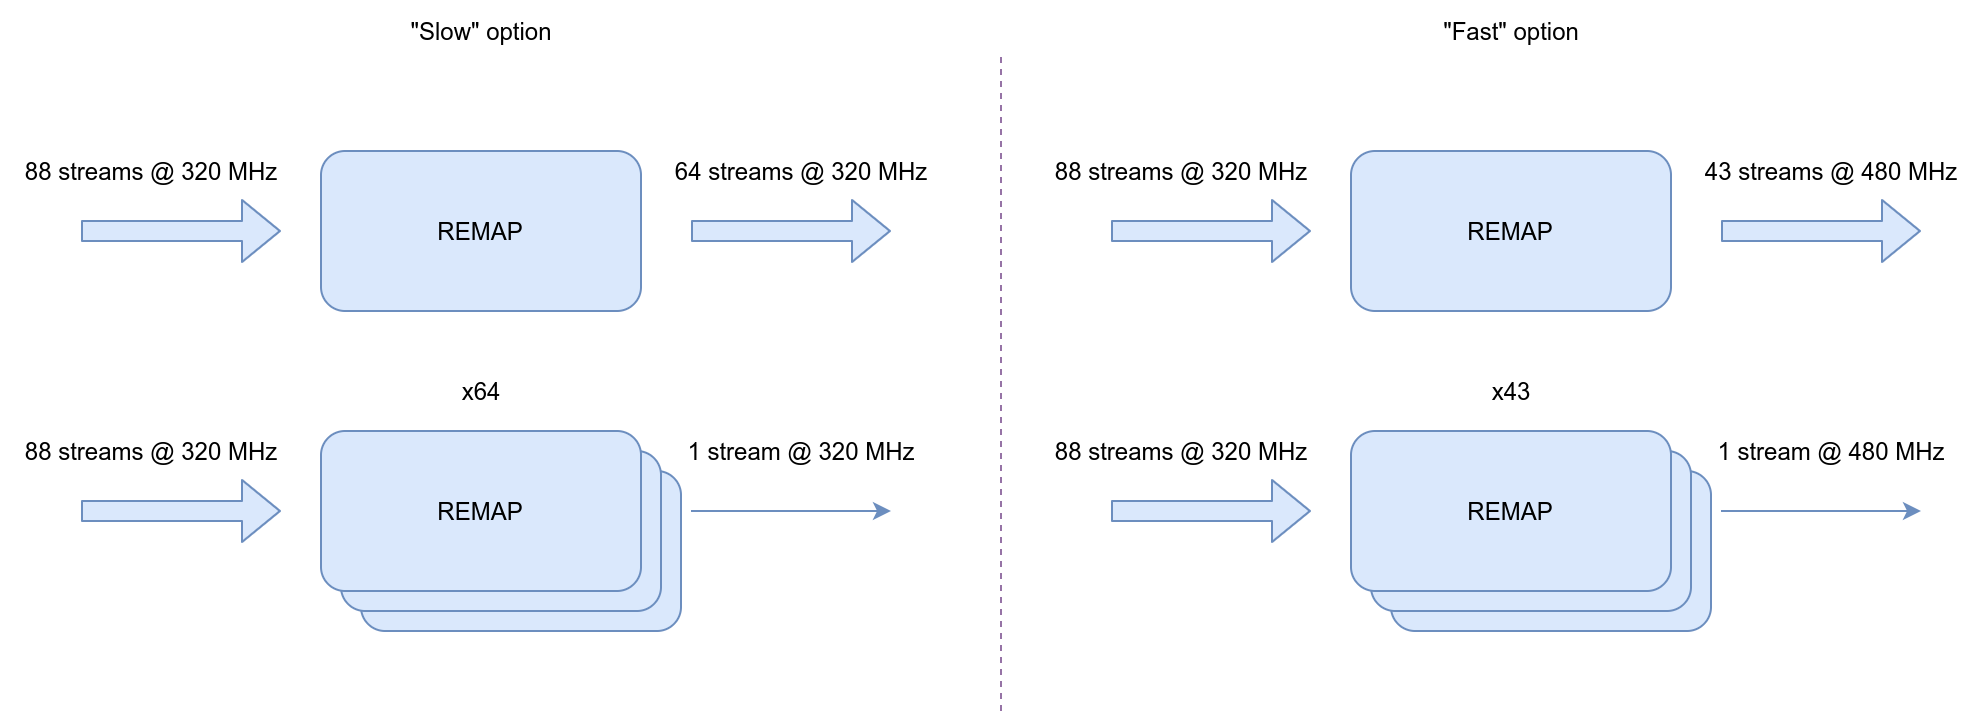
\includegraphics[width=\linewidth]{remap_replication.png}
    \caption{Схема формирования необходимого количества выходных каналов}
    \label{fig:remap_replication}
\end{figure}\par

Стоит отметить, поскольку входной поток данных разбивается на 4 независимые части, обрабатывающиеся отдельно, каждый модуль \texttt{remap} должен принимать лишь 22 канала и формировать 16 или 11 выходов, в зависимости от варианта сигнального процессора LASP.\par
В ходе разработки было спроектировано и реализовано два различных варианта архитектуры базового элемента модуля \texttt{remap}: с модулем синхронизации тактовых доменов, а также архитектура, основанная на FIFO памяти.\par
Во всех вариантах архитектуры можно выделить три основных этапа обработки:\par
\begin{itemize}
    \item предварительная перестановка данных в рамках каждого входного канала;
    \item извлечение из потока интересующих значений и их запись в память;
    \item чтение сохранённых данных из памяти в корректном порядке.
\end{itemize}\par
Первый этап обработки реализуется с помощью внешнего модуля Ialign и заключается в переупорядочивании значений АЦП в пределах каждого отдельного канала данных. Для корректной работы модуля \texttt{remap} требуется подобрать такую конфигурацию этих перестановок по всем каналам, чтобы значения, предназначенные для любого выходного канала не пересекались по временным ячейкам.\par
На втором этапе данные поступают на мультиплексор, который захватывает лишь один канал на каждом из тактов. Именно для этой операции и требуется условие первого этапа -- если одномоментно несколько входных каналов будут содержать значения, предназначенные для одного выходного, то часть данных будет просто пропущена. Это ограничение особенно важно для варианта сигнального процессора LASP с медленной опцией: как на входных интерфейсах, так и на выходных для каждого столкновения пучков передаётся по 8 величин, поэтому крайне необходимо, чтобы на каждом такте было доступно нужное значение. В быстрой опции выходной интерфейс имеет по 12 ячеек с данными, что вынуждает размещать два мультиплексора, ведь одного не будет достаточно в любом случае. В таком раскладе допускается одновременное наличие не более двух активных каналов для каждого базового блока модуля конфигурируемой перестановки. Извлечённые из общего потока значения, предназначенные для определённого выходного канала, временно буферизируются в памяти.\par
После накопления всех необходимых значений АЦП их необходимо переупорядочить, что осуществляется просто путём считывания данных в требуемой последовательности, согласно конфигурации. Стоит отметить, что буферизация данных в памяти позволяет обеспечить их безопасный переход из тактового домена $f_{feb}$ в домен $f_{core}$.\par

\subsubsection{Архитектура с модулем синхронизации тактовых доменов}
Первый вариант архитектуры компонента Remap, содержащий специальный модуль синхронизации тактовых доменов, представлен на рисунке \ref{fig:remap_cds}.\par
\begin{figure}[ht]
    \centering
    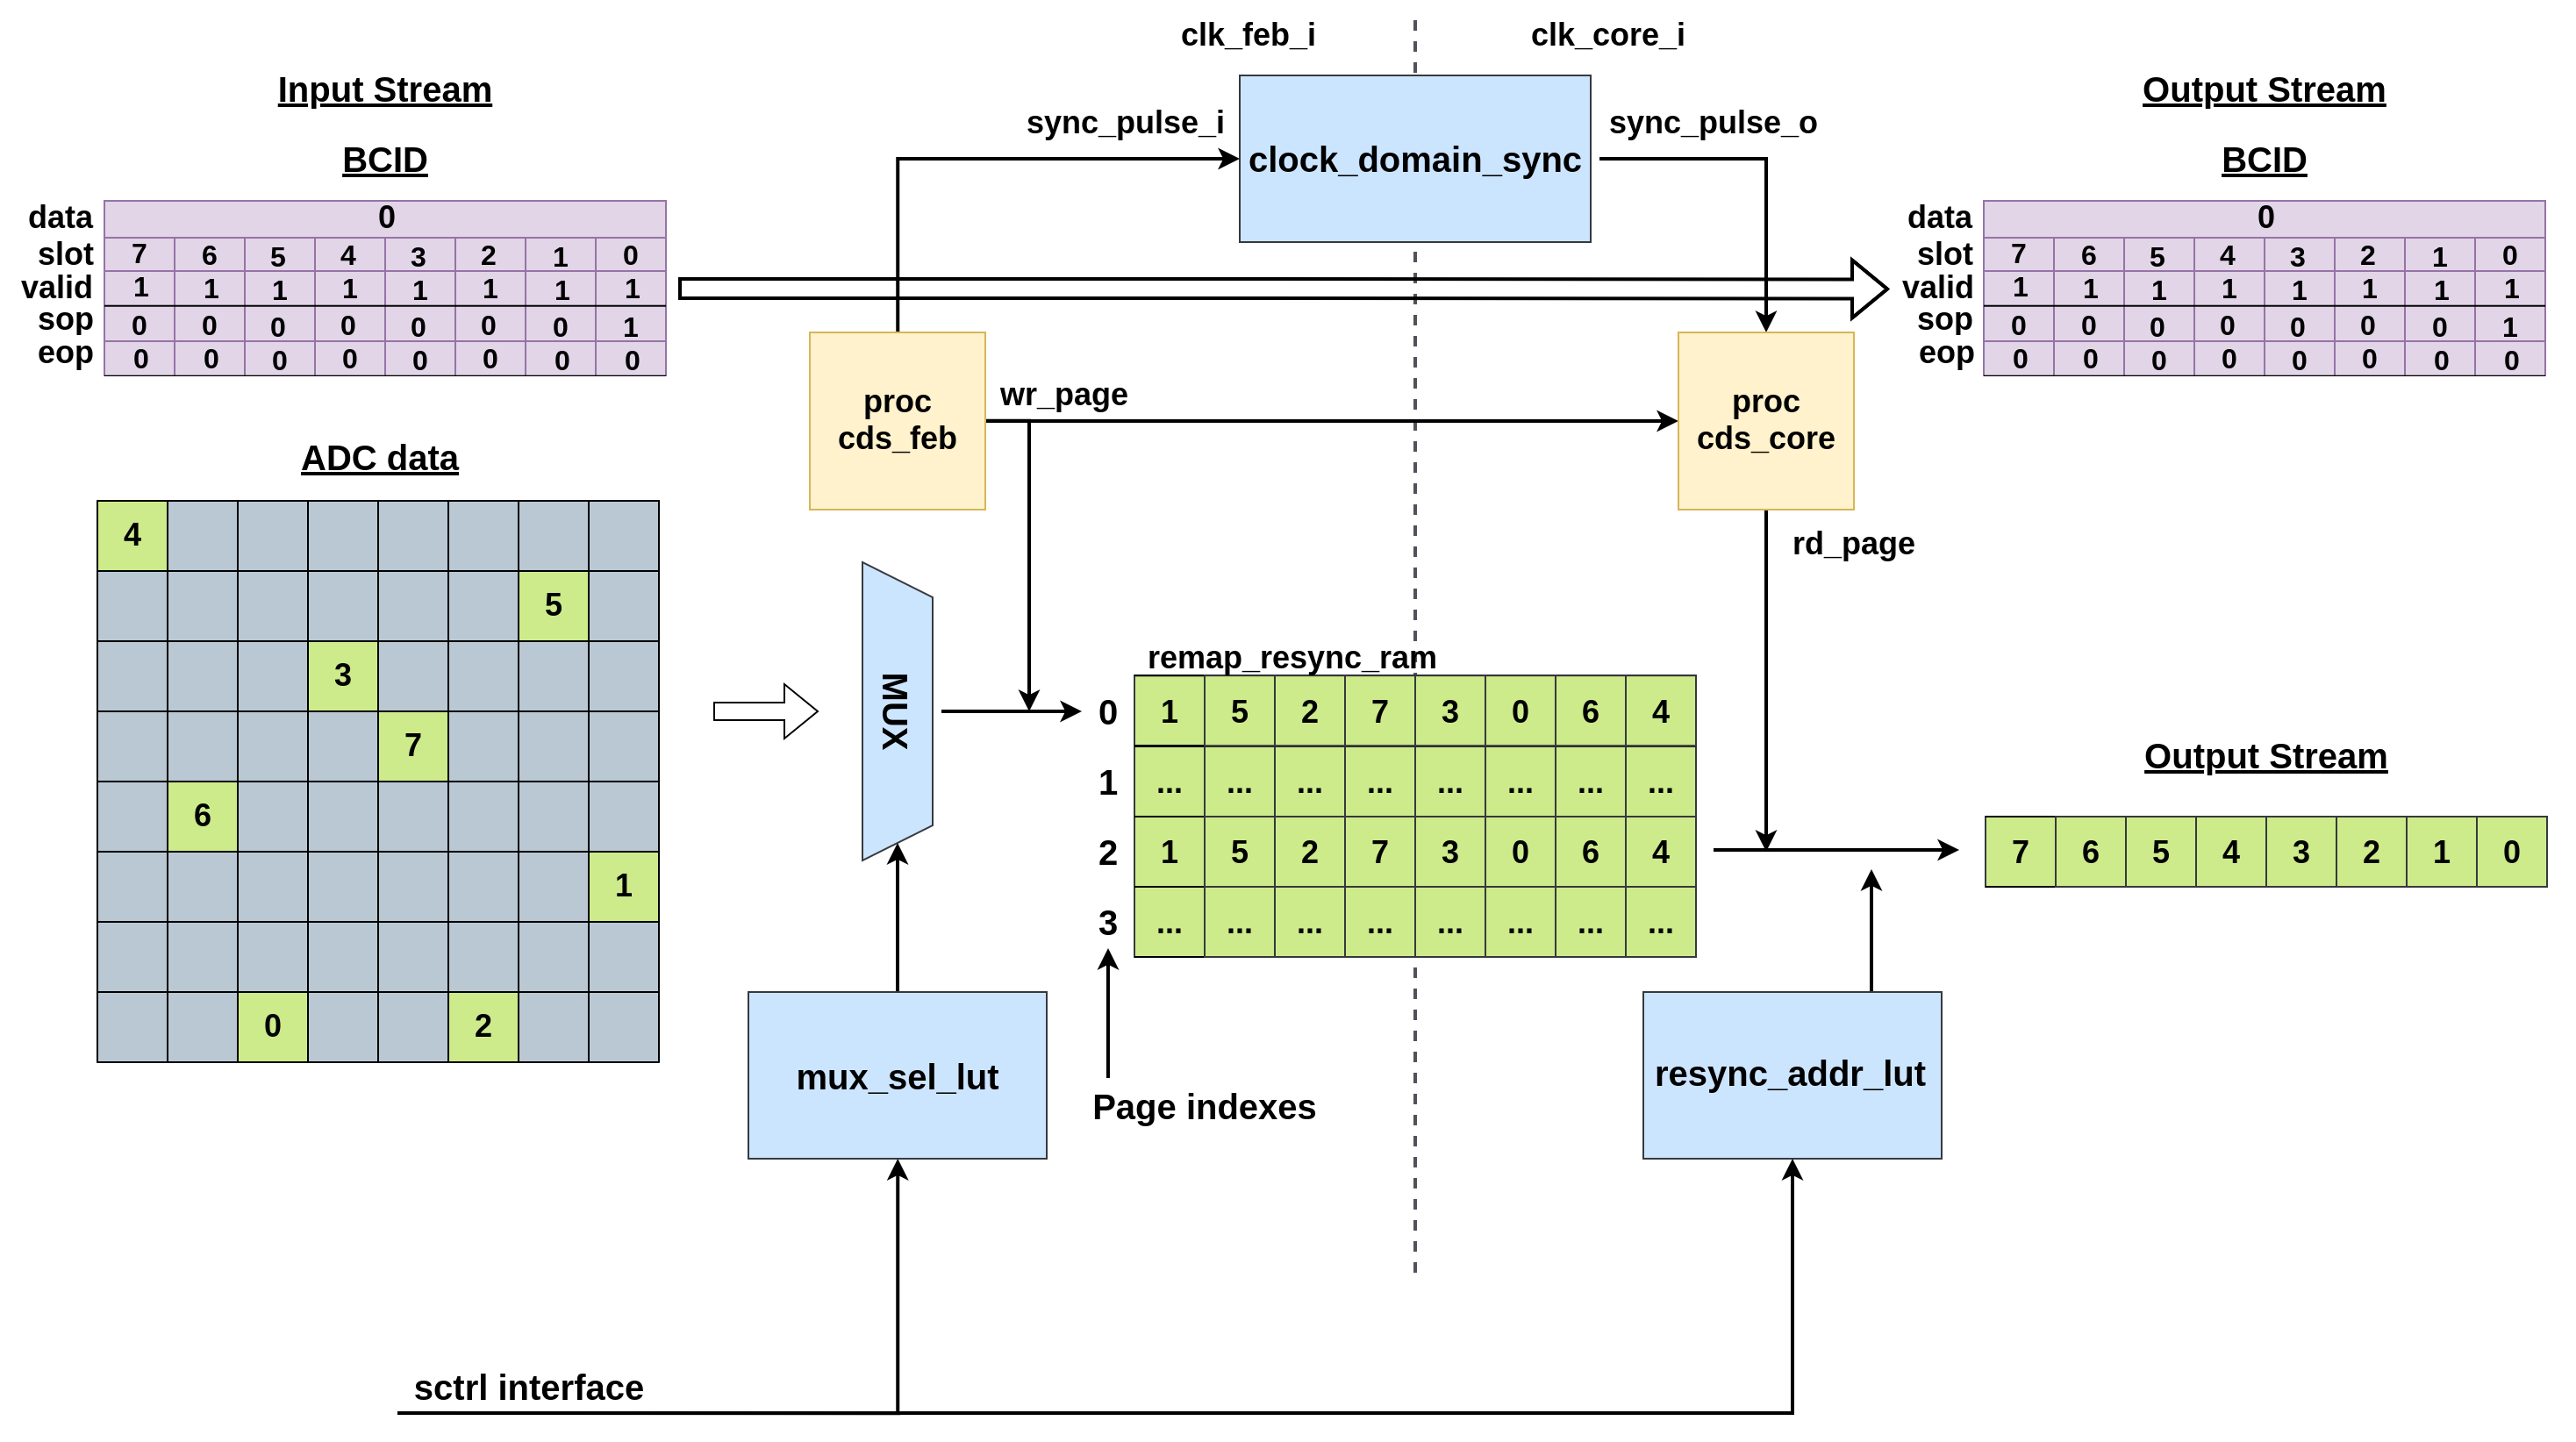
\includegraphics[width=\linewidth]{remap_cds.png}
    \caption{Схема архитектуры модуля Remap с модулем синхронизации тактовых доменов ПЕРЕВЕСТИ}
    \label{fig:remap_cds}
\end{figure}\par
Основной особенностью этой архитектуры является то, что в качестве буфера для мультиплексированных данных используется блок двухпортовой RAM памяти. Эта память разбита на несколько страниц, каждая из которых имеет размер, достаточный для хранения захваченной информации, относящейся к одному столкновению пучков. Чтение данных из страницы начинается лишь только после её полного заполнения записывающей стороной. Для синхронизации процессов считывания и записи предусмотрен следующий механизм: по завершению заполнения страницы памяти записывающая логика генерирует импульс шириной в один такт и отправляет его на вход специального модуля. Внутри этого модуля расположены два счётчика, работающие на тактовых частотах $f_{feb}$ и $f_{core}$, которые ведут счёт в диапазоне количества временных ячеек для каждого BCID. В рабочем режиме первый настроен так, чтобы обнуляться одновременно с поступлением синхросигнала от записывающей логики, а второй с задержкой около такта $f_{feb}$ после первого. При завершении цикла работы второго счётчика формируется выходной сигнал синхронизации, который поступает к считывающей логике и означает, что очередная страница в двухпортовой памяти заполнена полностью и можно безопасно извлекать из неё данные. Если вдруг синхронизация собьётся и синхросигнал от системы записи придёт не вовремя, то модуль это обнаружит и перейдёт в режим восстановления синхронизации. Часть данных после сбоя синхронизации будет утеряно, но через некоторое время система автоматически восстановится и продолжит работать исправно.\par
Описанная архитектура была реализована на языке описания цифровой логики VHDL и отлажена. По результатам тестирования в симуляторе она подтвердила свою работоспособность. Однако такой подход имеет ряд недостатков, главным из которых является необходимость передавать целый набор сигналов(такие как номер текущей страницы, индекс столкновения пучка, а также ряд вспомогательных сигналов внутри модуля синхронизации тактовых доменов) между тактовыми доменами $f_{feb}$ и $f_{core}$ вручную, используя схемы на двух регистрах. Для корректной организации таких переходов требуется тонкая ручная настройка временных ограничений, реализуемая путём составления специальных указаний синтезатору физической схемы, входящему в состав программного комплекса Intel Quartus Prime. Это значительно усложняет весь проект и делает его гораздо менее гибким. После возникновения проблем с разводимостью логики проекта LATOME, который является основой задетекторной электроники эксперимента ATLAS, разработанной в рамках предшествующей фазы обновления детектора, командой разработчиков сигнального процессора LASP было принято решение максимально избегать подобные способы перехода между тактовыми доменами. Кроме того, данный вариант является довольно путанным и сложным для понимания в деталях. Учитывая все эти недостатки, было решено разработать альтернативную архитектуру модуля Remap.\par


\subsubsection{Архитектура, основанная на FIFO}
Второй вариант архитектуры компонента Remap, содержащий память FIFO, представлен на рисунке \ref{fig:remap_fifo}.\par
\begin{figure}[ht]
    \centering
    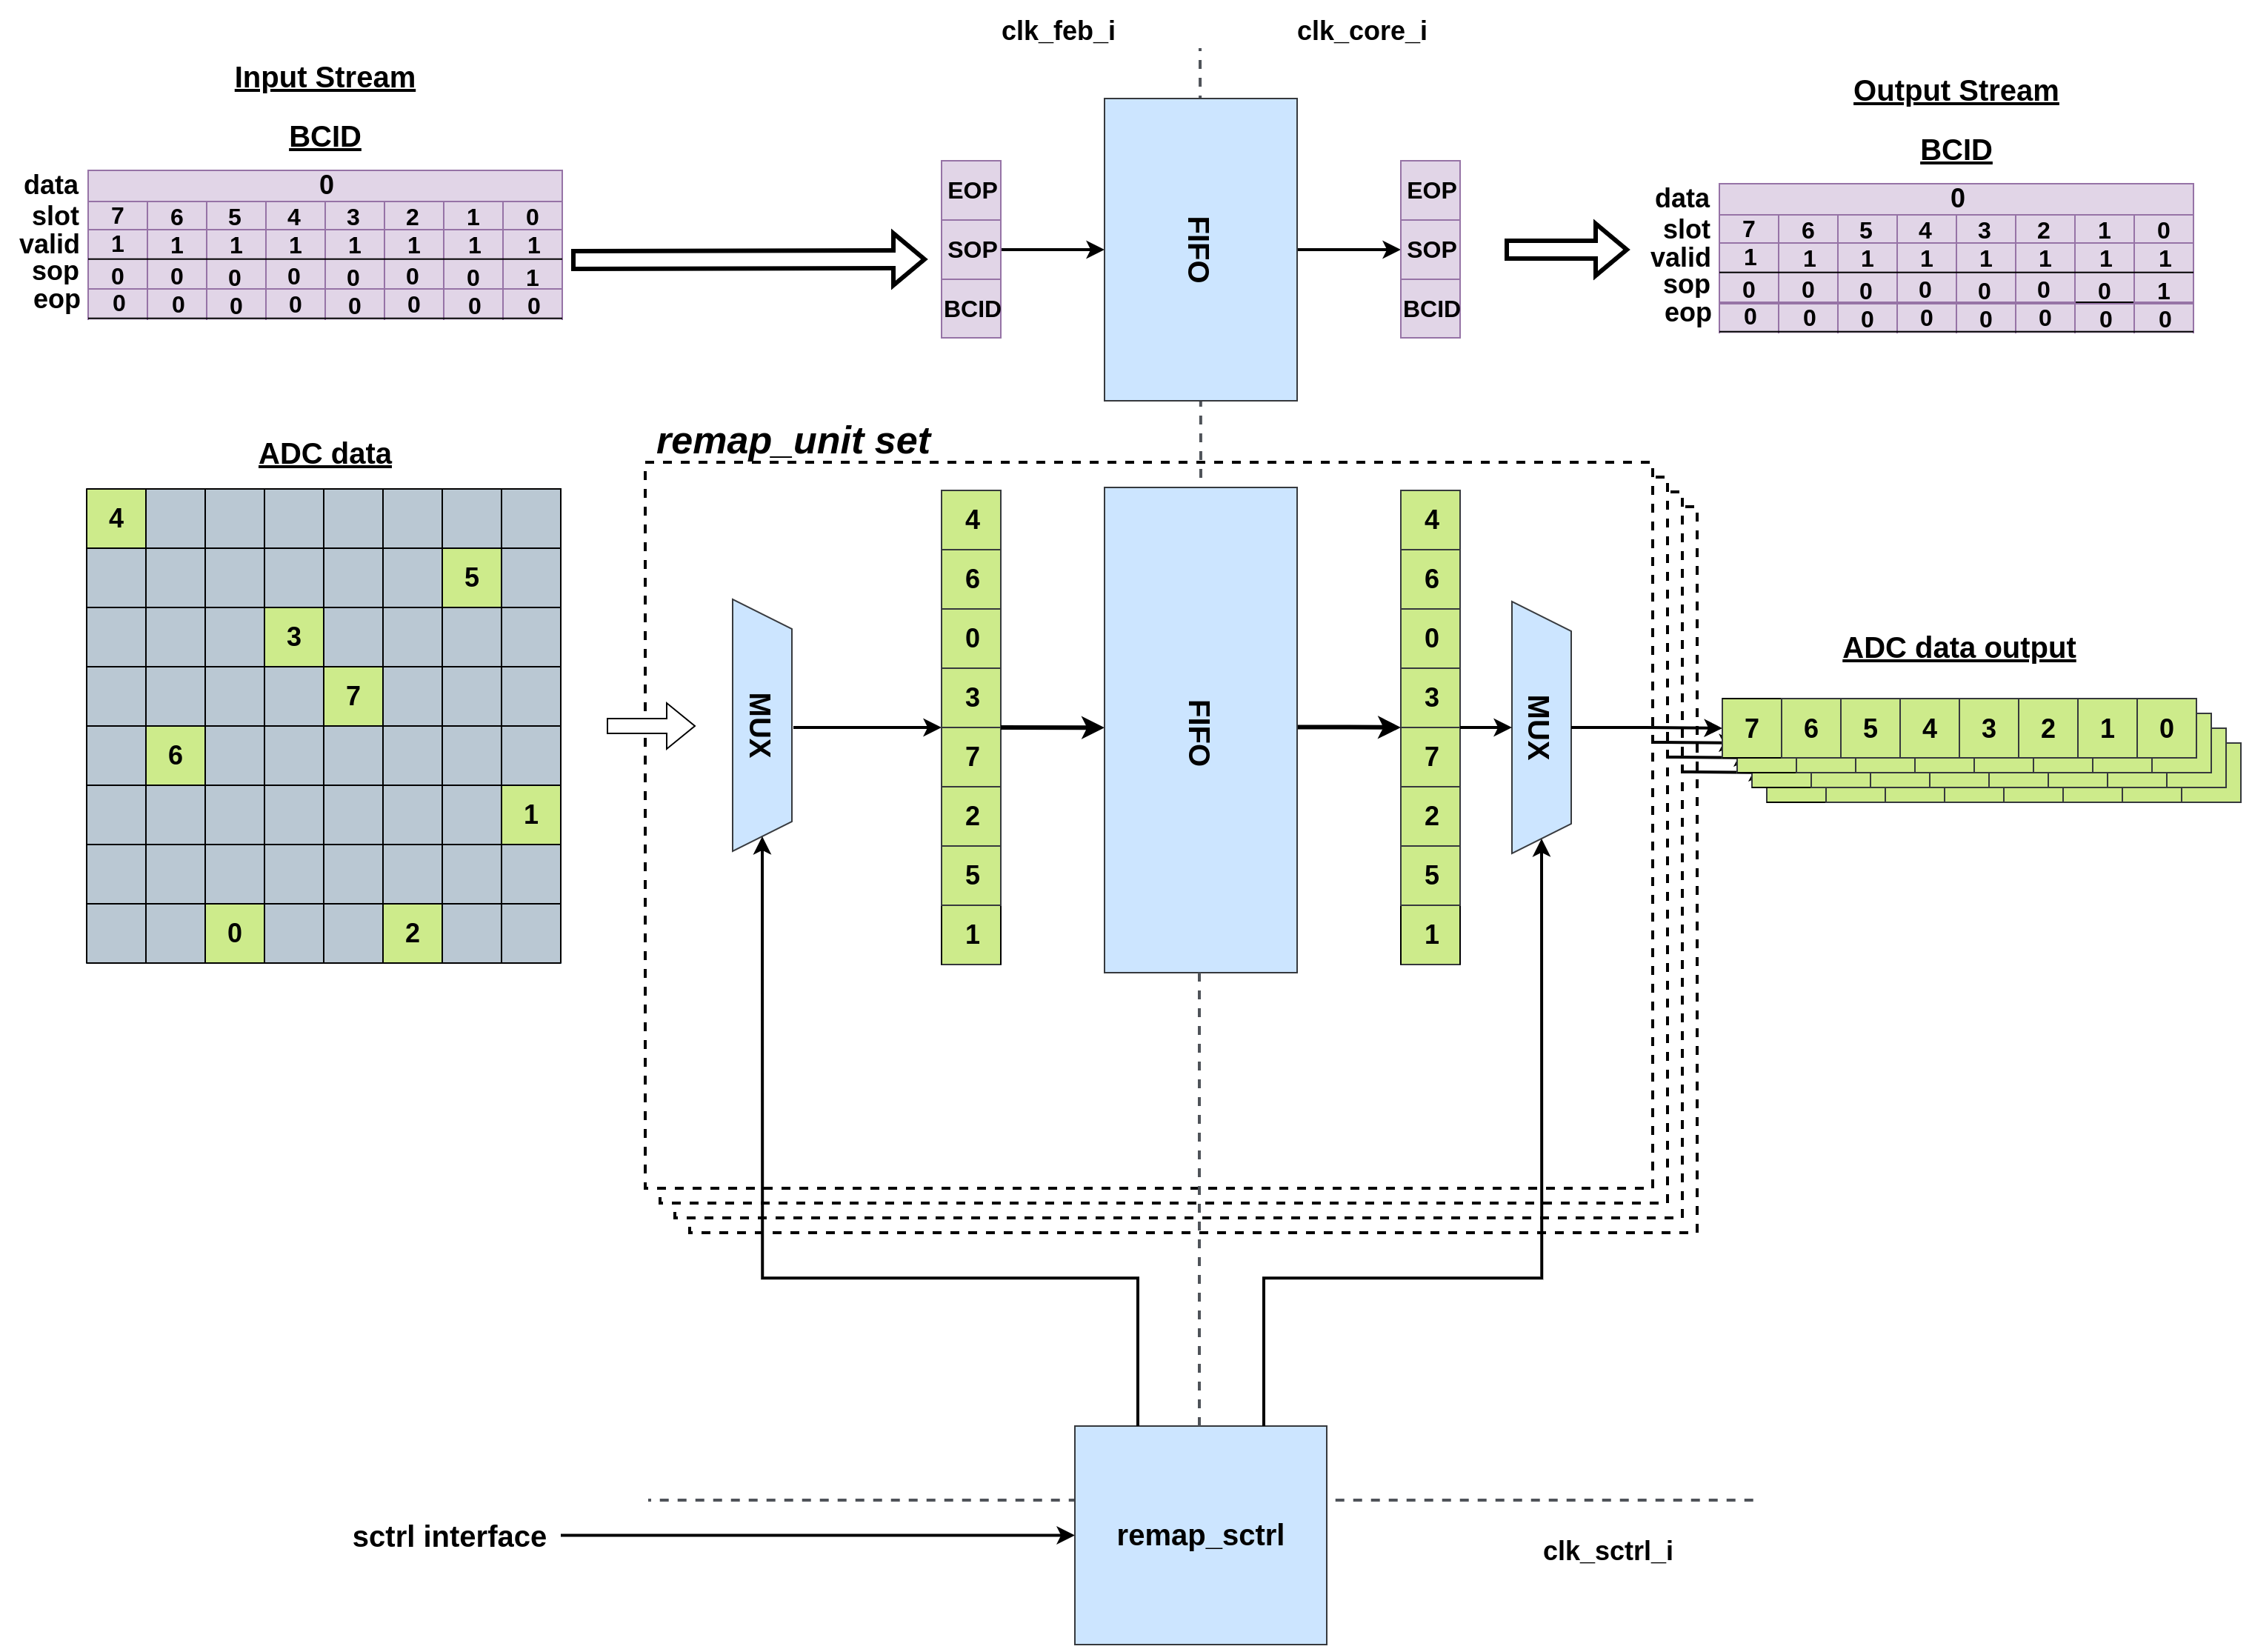
\includegraphics[width=\linewidth]{remap_fifo.png}
    \caption{Схема архитектуры модуля Remap, основанной на FIFO ПЕРЕВЕСТИ}
    \label{fig:remap_fifo}
\end{figure}\par
В рамках данного подхода в качестве буфера для мультиплексированных данных является память FIFO (First In First Out). Такая структура состоит из двухпортовой памяти, двух счётчиков адреса и двух автоматов для чтения и записи данных и является одним из ключевых элементов цифровой схемотехники. Одно из самых распространённых применений такой памяти, помимо буферизации информации -- это реализация перехода данных между тактовыми доменами. Поскольку такая память используется невероятно часто в проектировании логических схем, то существует множество готовых вариантов их реализации, в том числе и от разработчиков самих микросхем ПЛИС и соответствующего программного обеспечения для автоматического проектирования, в том числе и от Intel. В случае использования такого готового блока FIFO не требуется ручное написание временных ограничений, что избавляет от потенциальных проблем на этапе синтеза цифровой схемы всего проекта.\par
Однако, одна из основных особенностей FIFO -- это сохранение порядка записываемых данных, что не позволяет реализовать последний этап работы модуля Remap. Для решения данной задачи используется подход, при котором данные с мультиплексора поступают не напрямую на вход FIFO, а записываются в один большой регистр, достаточного размера для одновременного хранения всех мультиплексированных данных в рамках текущего столкновения пучков. Для наиболее оптимального использования логических ресурсов этот регистр является сдвиговым, то есть каждый такт новое значение поступает в начало, после чего оно смещается дальше. Только после полного заполнения этого регистра актуальными величинами, данные одним большим словом записывается в FIFO. Считывающая логика, после обнаружения данных на выходе FIFO, имеет доступ сразу ко всем значениям и может извлекать их последовательно в необходимом порядке.\par
В целях минимизации латентности необходимо, чтобы поступающие в FIFO данные сразу же были доступны для чтения, то есть требуется не допускать его заполнения. Поскольку запись и извлечение идёт с одной и той же скоростью, важно важно сделать так, чтобы считывающая система начала работу как минимум не позднее записывающей. Это достигается правильным управлением сигналами сброса: после старта сигнального процессора LASP сначала должен сняться сброс, синхронный с тактовым доменом $f_{core}$, а уже затем $f_{feb}$.\par



\subsection{Конфигурирование через интерфейс медленного контроля}
Конфигурирование модуля \texttt{remap} осуществляется через интерфейс медленного контроля. Как упоминалось ранее, он функционирует поверх протокола Avalon Memory Mapped, который предназначен для работы с адресуемой памятью. Такой подход очень удобен, поскольку в этом случае можно выделить каждому модулю свой участок адресов, по которым можно будет располагать необходимые значения. Разные адреса можно настроить по способу доступа к ним, таким образом можно завести некоторые показатели системы, которые можно будет только считывать, или же добавить параметры с опцией модификации. Отдельная важная особенность работы через память -- возможность функционирования в разных тактовых доменах, для этого достаточно использовать модули двухпортовой памяти. Это позволяет использовать достаточно низкую тактовую частоту для интерфейса конфигурации, чтобы он не оказывал существенного влияния на разводимость остальной логики. Причём эта частота может быть единой для конфигурирования всех компонентов, вне зависимости от их внутренних тактовых сигналов, что значительно упрощает работу медленного контроля.\par
Модуль перестановки \texttt{remap} имеет две конфигурируемые стадии: какие значения извлекать из общего потока данных с помощью мультиплексора и в каком порядке их выдавать в выходной канал. Поскольку эти стадии работают в разных тактовых доменах, то необходимо размещать параметры для них в разных блоках памяти, чтобы можно было корректно переводить значения в целевые тактовые частоты. Начальный адрес конфигурации мультиплексора устанавливается глобальной константой REMAP\_BADDR (Remap Base Address) с уровня всего проекта сигнального процессора LASP, а конфигурация порядка выходных данных имеет некоторое смещение относительно него. На рисунке \ref{fig:remap_sctrl_mapping} изображена схема отображения конфигураций на адресное пространство.\par
\begin{figure}[ht]
    \centering
    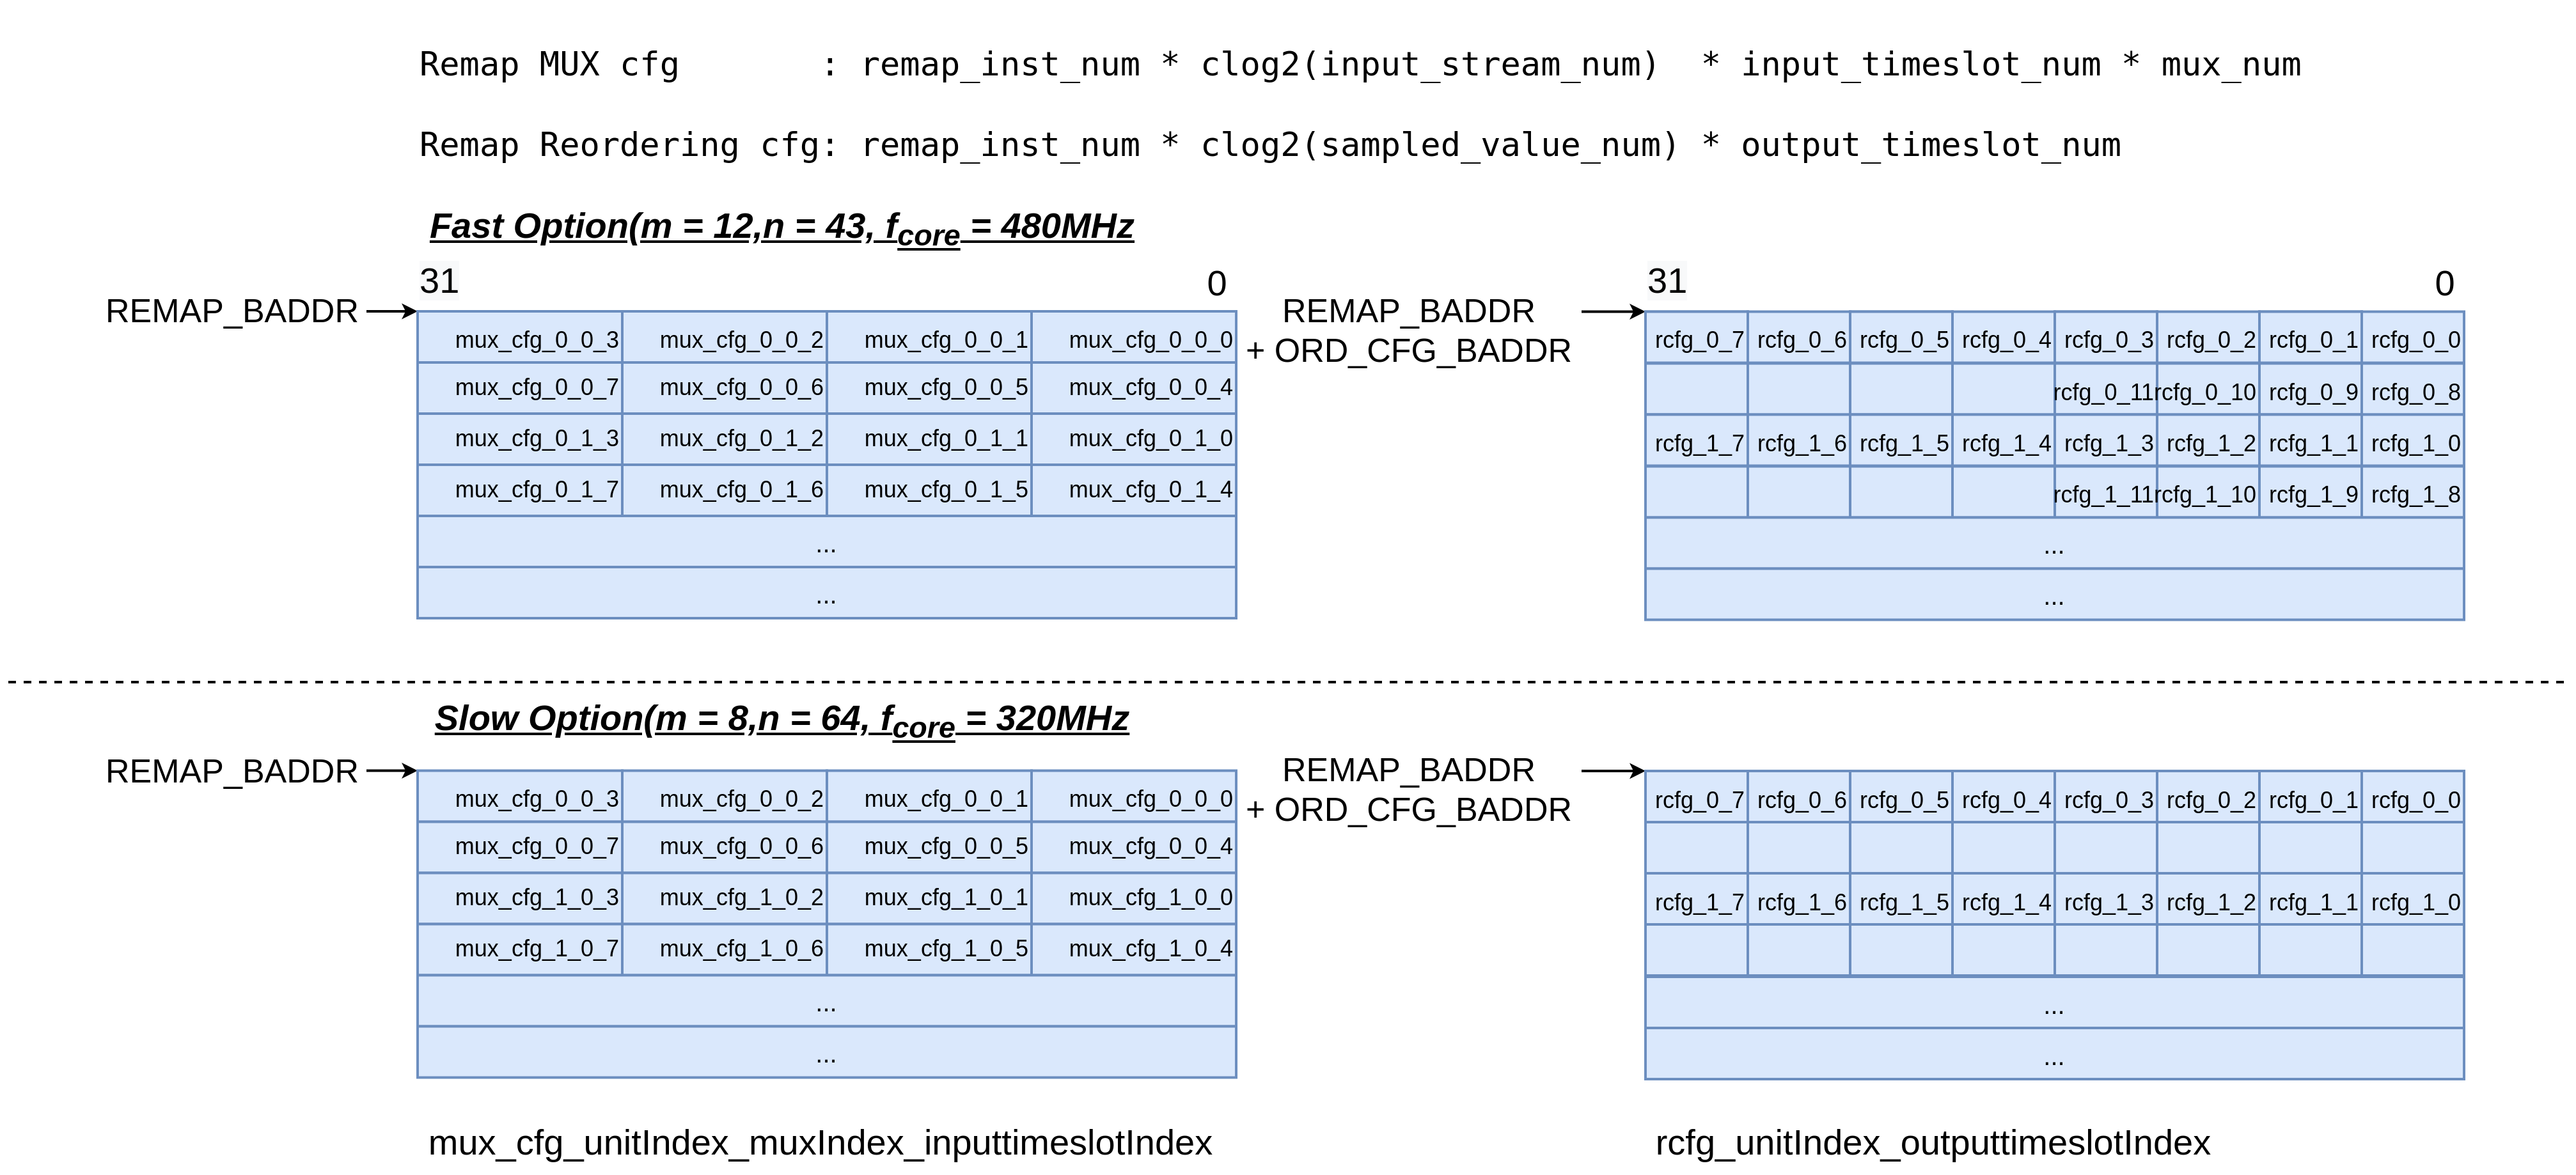
\includegraphics[width=\linewidth]{remap_sctrl_mapping.png}
    \caption{Схема маппинга памяти модуля перестановки \texttt{remap} для записи конфигурации}
    \label{fig:remap_sctrl_mapping}
\end{figure}\par
Для конфирурирования входного мультиплексора необходимо для каждой временной ячейки установить номер канала, с которого необходимо захватить данные. На каждый \texttt{remap} поступает по 22 канала, то есть требуется 5 бит на значение. Для любого столкновения пучков выделяется по 8 временных интервалов, следовательно суммарно должно быть не менее 40 бит данных для конфигурирования одного выходного канала \texttt{remap}. Шина данных интерфейса Avalon Memory Mapped имеет ширину 32 бита, поэтому для удобства формирования и чтения конфигурационных данных используется 2 слова AVMM, что составляет 64 бита. В случае варианта быстрой опции сигнального процессора LASP требуется два входных мультиплексора, соответственно размер конфигурации удваивается и равняется 128 бит.\par
Конфигурирование финальной перестановки осуществляется путём последовательного указания индекса необходимого значения. В зависимости от медленной или быстрой опции отобранных величин может быть 8 или 16 соответственно. Для более удобной работы под каждое такое значение выделяется по 4 бита. Далее, в зависимости от варианта сигнального процессора LASP требуется от 8 до 12 временных ячеек для каждого BCID, следовательно суммарно необходимо иметь от 32 до 48 бит. Аналогично конфигурации мультиплексора, в целях повышения удобства размер конфигурации округляется по ширине шины интерфейса AVMM и составляет 64 бита независимо от опции сигнального процессора LASP.\par


\subsection{Реализация}
В ходе реализации синтезируемых компонентов модуля Remap активно использовалось тестирование с помощью симуляции. Оно осуществлялось с помощью специализированного программного обеспечения Mentor QuestaSim, предназначенное для моделирования и отладки микросхем ПЛИС. Симуляционное окружение разработано, как и синтезируемые модули, на языке VHDL и обеспечивает поступление данных на входной интерфейс тестируемого модуля. Так, на рисунке \ref{fig:sim_input} приведён фрагмент симуляции, на котором показан пример данных внутри внутри  входного интерфейса. Можно увидеть, что как и в реальной системе, в каждый модуль Remap поступает 22 канала со значениями АЦП, причем для каждого BCID передаётся по 8 величин в канале. Все сигналы входного сигнала синхронны с тактовой частотой $f_{feb}$.\par
\begin{figure}[ht]
    \centering
    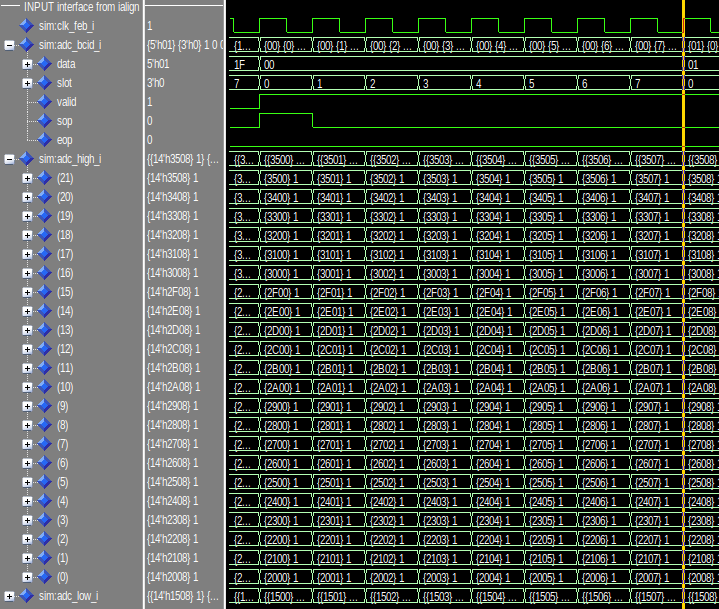
\includegraphics[width=\linewidth]{sim_input.png}
    \caption{Фрагмент поступающих в модуль Remap входных данных в симуляции ВЗЯТЬ МАСШТАБ ПОКРУПНЕЙ}
    \label{fig:sim_input}
\end{figure}\par
В рассматриваемом примере модуль предназначен для работы в варианте сигнального процессора LASP с установленной медленной опцией. В качестве конфигурации производится установка параметров для первых двух выходных каналов Remap компонента. На рисунке \ref{fig:sim_sctrl} отображено, как это осуществляется через интерфейс медленного контроля. На волновой диаграмме отчетливо видно, как значения поступают в установленном формате по протоколу AVMM, после чего лишние биты отсекаются, а сами конфигурационные данных переходят в соответствующие им тактовые домены. В соответствии с настройкой, первый выходной канал должен выдавать данные из первых восьми входных каналов в обратной последовательности, а второй по четыре значения из каналов с номерами 20 и 21 в чередующейся последовательности.\par
\begin{figure}[ht]
    \centering
    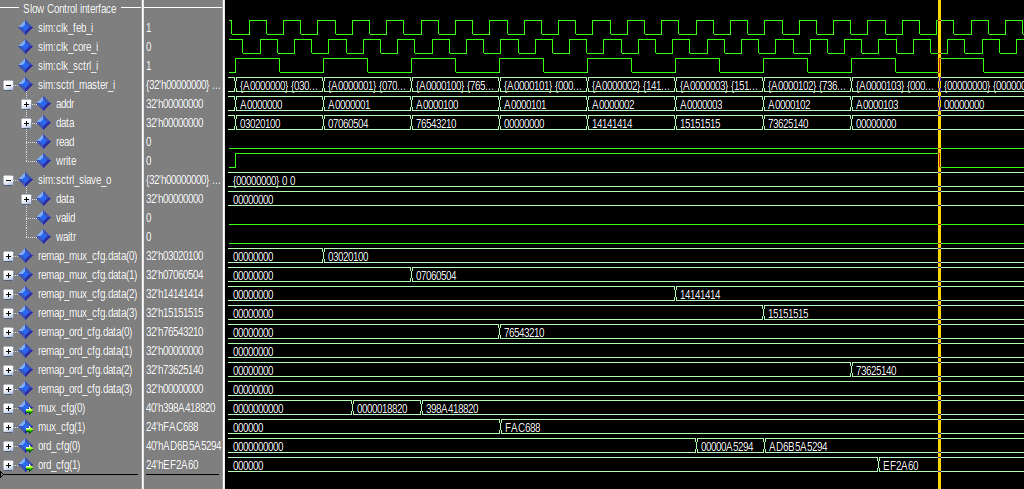
\includegraphics[width=\linewidth]{sim_sctrl.png}
    \caption{Пример записи конфигурации модуля Remap в симуляции}
    \label{fig:sim_sctrl}
\end{figure}\par
На рисунке \ref{fig:sim_output} изображен выходной интерфейс модуля конфигурируемой перестановки. Поскольку система предназначена для работы в медленной опции сигнального процессора LASP, выходной интерфейс состоит из 16 каналов, в котором данные передаются синхронно частоте $f_{core}$, равной 320 МГц. На нём можно отследить корректность работы компонента, работающего в соответствии с вышеописанными настройками. \par
\begin{figure}[ht]
    \centering
    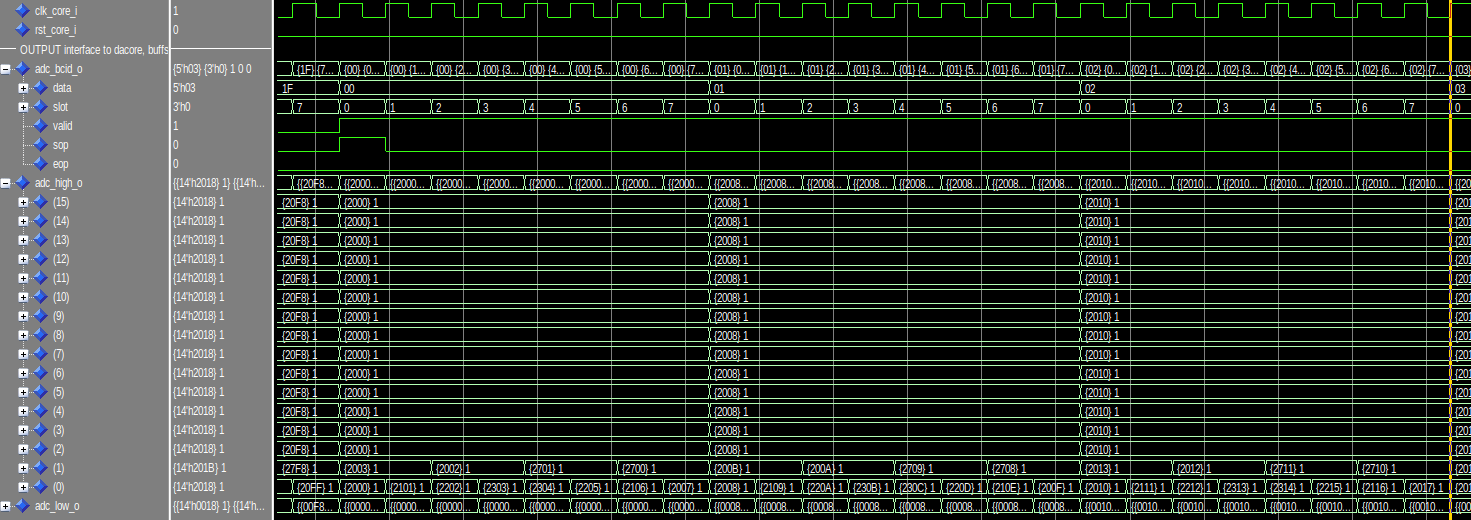
\includegraphics[width=\linewidth]{sim_output.png}
    \caption{Фрагмент выходящих из модуля Remap данных в симуляции ВЗЯТЬ МАСШТАБ ПОКРУПНЕЙ}
    \label{fig:sim_output}
\end{figure}\par


    \newpage

\section{Модуль упаковки данных (Packer)}
    Модуль \texttt{packer} является частью сигнального процессора LASP и предназначен для вычисления необходимых энергетических сумм по узлам калориметра и последующей упаковки данных для отправки в целевую систему.\par
\begin{figure}[ht]
    \centering
    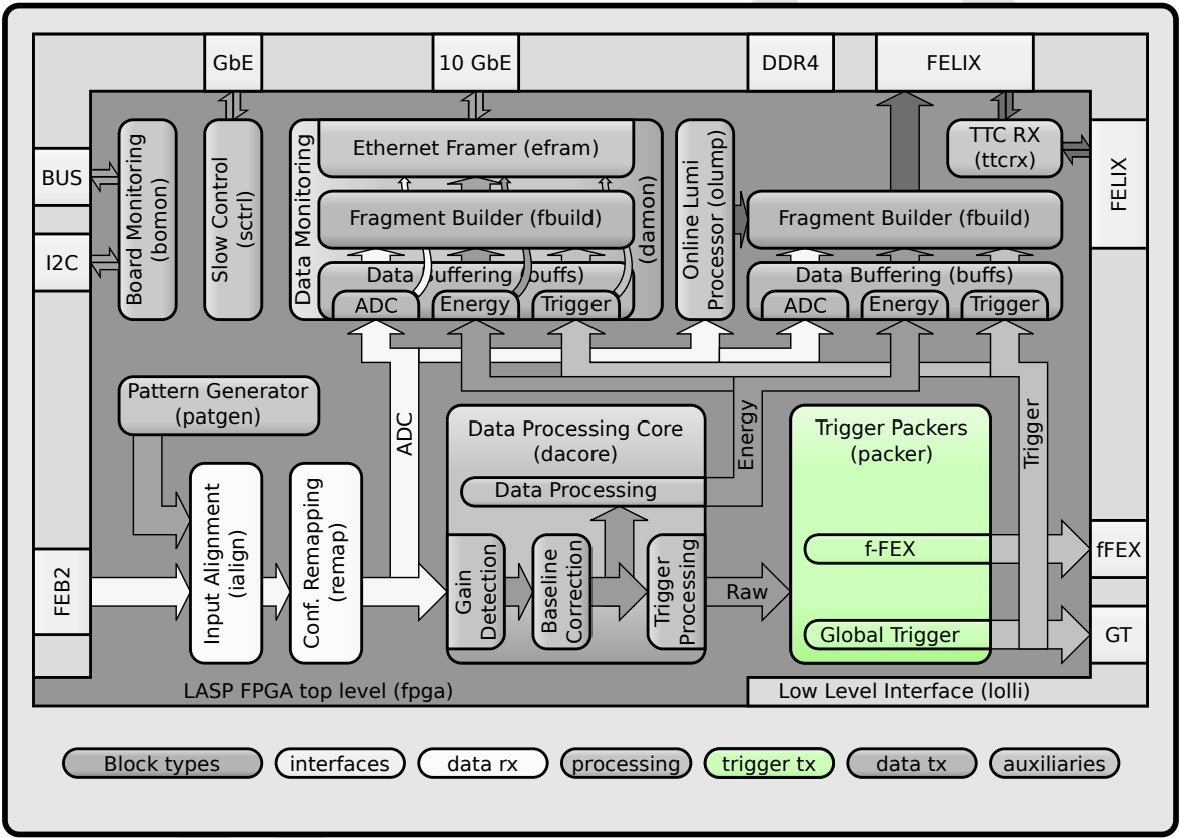
\includegraphics[width=0.8\linewidth]{packer_lasp.png}
    \caption{Схема расположения модуля packer в общей структуре сигнального процессора LASP}
    \label{fig:packer_lasp}
\end{figure}\par

Модуль \texttt{packer} обеспечивает данные для двух внешних подсистем: глобальный триггер и fFEX. Система fFEX \parencite{tdr_blue} является представителем набора модулей FEX, с помощью которых осуществляется поиск специфичных событий в ускорителе. Для этого ей не требуется полный объём данных, поступающих с детектора, а достаточно лишь определённой части, причём зачастую используются не конкретные значения, а суммы по целым участкам калориметра.\par
Для передачи данных во внешние подсистемы используется подход упаковки информации в кадры, которые уже непосредственно отправляются клиенту. Поскольку в системе сбора данных имеется жесткая система синхронизации -- приёмник и передатчик синхронизованы между собой и частотой БАК -- при передаче данных не требуется синхронизация в каждом пакете. Полоса пропускания полностью используется для передачи данных, упакованных в кадры, в каждом из которых содержатся данные от одного столкновния пучков. На рисунке \ref{fig:packer_ffex_frame} изображен один из предложенных вариантов формата кадра данных. Он содержит 46 десятибитных значений АЦП, идентификатор столкновения пучков, а также флаги превышения данными порога $2 \sigma$. Помимо представленного варианта также были предложения реализовать кадры с переменной структурой, которые наиболее эффективно использовали бы пропускную способность канала передачи данных для разных участков калориметра.\par
\begin{figure}[ht]
    \centering
    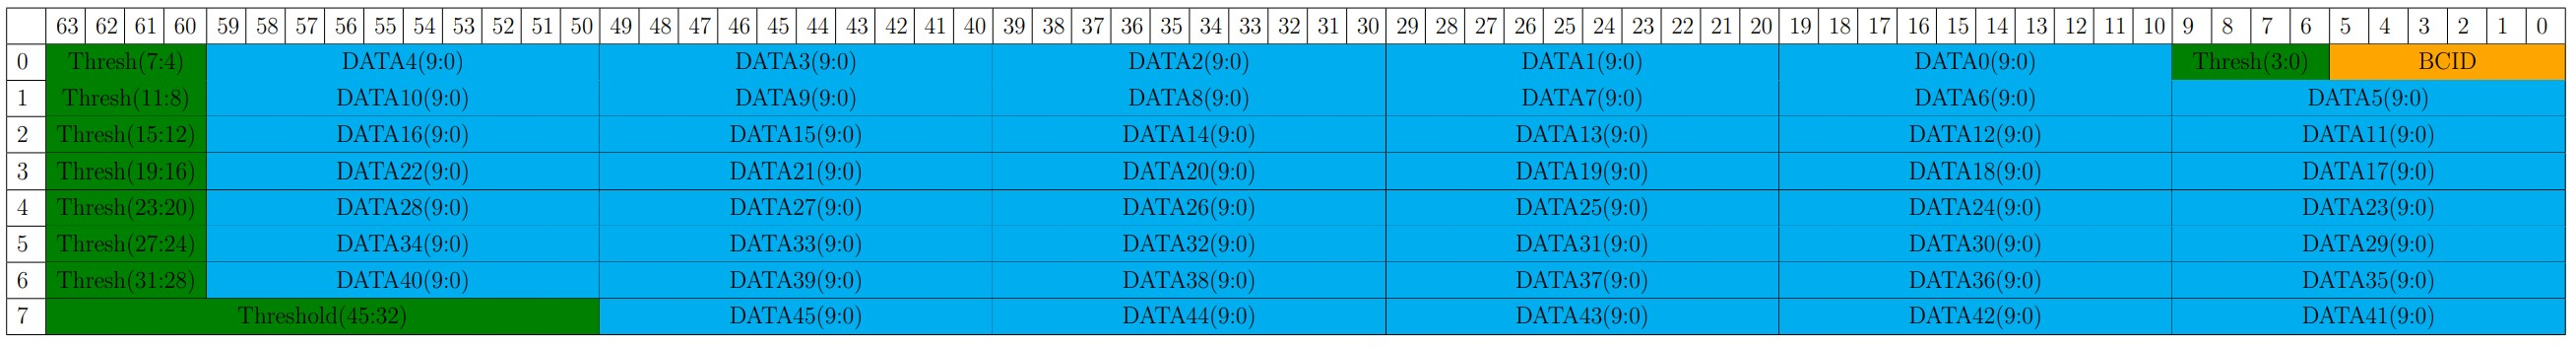
\includegraphics[width=\linewidth]{packer_ffex_frame.png}
    \caption{Вариант формата кадра данных для отправки в систему fFEX}
    \label{fig:packer_ffex_frame}
\end{figure}\par
В ходе работы был разработан прототип модуля \texttt{packer} на языке описания цифровой логики VHDL, и подготовлено тестовое симуляционное окружение для моделирования его поведения. Также этот модуль был интегрирован в общий дизайн сигнального процессора LASP в рамках подхода top-down \parencite{topdown}. Таким образом, весь дизайн целиком LASP сейчас может модулироваться и компилироваться. Целевая функциональность модуля упаковки триггерных данных будет реализована после согласования требований с разработчиками системы fFEX (ожидается в 2023).\par

\newpage

\section*{Заключение}
\addcontentsline{toc}{section}{Заключение}
    В рамках данной работы велась разработка блока упаковки данных сигнального процессора жидкоаргоновых калориметров LASP для системы FEX, состоящей из связки модулей конфигурируемой перестановки \texttt{remap} и упаковщика триггерных данных \texttt{packer}. Таким образом, были реализованы следующие задачи:\par
\begin{itemize}
    \item по модулю конфигурируемой перестановки \texttt{remap}:
        \begin{itemize}
            \item проработана внутренняя архитектура -- составлено 2 альтернативных варианта;
            \item написаны синтезируемые блоки цифровой логики на языке VHDL;
            \item создано симуляционное окружение для моделирования поведения модуля;
            \item проведена компиляция под целевую платформу;
            \item выполнена интеграция модуля в основную структуру сигнального процессора LASP;
            \item разработан прототип программного обеспечения для автоматической генерации конфигурации;
        \end{itemize}
    \item по упаковщику триггерных данных \texttt{packer} для системы fFEX:
        \begin{itemize}
            \item разработаны протоколы упаковки данных в кадры;
            \item реализован синтезируемый прототип модуля;
            \item создано симуляционное окружение для моделирования поведения модуля;
            \item выполнена интеграция модуля в основную структуру сигнального процессора LASP.
        \end{itemize}
\end{itemize}\par
В дальнейшем планируется масштабирование программного обеспечения для автоматической генерации конфигураций модуля \texttt{remap} на все участки жидкоаргонового калориметра. После согласования требований с разработчиками системы fFEX будет завершена реализация упаковщика \texttt{packer}. После завершения разработки предстоит запуск систем на целевой платформе и последующий ввод в эксплуатацию.\par

    \newpage

%\inputencoding{T2A}
%\usepackage[koi8-r]{inputenc}
%\bibliographystyle{utf8gost705u}
\printbibliography
%\printbibliography{sections/bibliography}
%\inputencoding{utf8}

\addcontentsline{toc}{section}{Список литературы}
\end{document}
